\documentclass[a4paper]{article}

\def\npart {IB}
\def\nterm {Lent}
\def\nyear {2016}
\def\nlecturer {A.\ G.\ Kovalev}
\def\ncourse {Geometry}

\usepackage{myheader}

\begin{document}
\maketitle
{\small
\noindent\emph{Parts of Analysis II will be found useful for this course.}
\vspace{10pt}

\noindent Groups of rigid motions of Euclidean space. Rotation and reflection groups in two and three dimensions. Lengths of curves.\hspace*{\fill} [2]

\vspace{5pt}
\noindent Spherical geometry: spherical lines, spherical triangles and the Gauss-Bonnet theorem. Stereographic projection and M\"obius transformations.\hspace*{\fill} [3]

\vspace{5pt}
\noindent Triangulations of the sphere and the torus, Euler number.\hspace*{\fill} [1]

\vspace{5pt}
\noindent Riemannian metrics on open subsets of the plane. The hyperbolic plane. Poincar\'e models and their metrics. The isometry group. Hyperbolic triangles and the Gauss-Bonnet theorem. The hyperboloid model.\hspace*{\fill} [4]

\vspace{5pt}
\noindent Embedded surfaces in $\R^3$. The first fundamental form. Length and area. Examples.\hspace*{\fill} [1]

\vspace{5pt}
\noindent Length and energy. Geodesics for general Riemannian metrics as stationary points of the energy. First variation of the energy and geodesics as solutions of the corresponding Euler-Lagrange equations. Geodesic polar coordinates (informal proof of existence). Surfaces of revolution.\hspace*{\fill} [2]

\vspace{5pt}
\noindent The second fundamental form and Gaussian curvature. For metrics of the form $du^2 + G(u, v) dv^2$, expression of the curvature as $\sqrt{G_{uu}}/\sqrt{G}$. Abstract smooth surfaces and isometries. Euler numbers and statement of Gauss-Bonnet theorem, examples and applications.\hspace*{\fill} [3]}

\tableofcontents
\setcounter{section}{-1}
\section{Introduction}
In the very beginning, Euclid came up with the axioms of geometry, one of which is the \emph{parallel postulate}. This says that given any point $P$ and a line $\ell$ not containing $P$, there is a line through $P$ that does not intersect $\ell$. Unlike the other axioms Euclid had, this was not seen as ``obvious''. For many years, geometers tried hard to prove this axiom from the others, but failed.

Eventually, people realized that this axiom \emph{cannot} be proved from the others. There exists some other ``geometries'' in which the other axioms hold, but the parallel postulate fails. This was known as \emph{hyperbolic geometry}. Together with Euclidean geometry and spherical geometry (which is the geometry of the surface of a sphere), these constitute the three classical geometries. We will study these geometries in detail, and see that they actually obey many similar properties, while being strikingly different in other respects.

That is not the end. There is no reason why we have to restrict ourselves to these three types of geometry. In later parts of the course, we will massively generalize the notions we began with and eventually define an \emph{abstract smooth surface}. This covers all three classical geometries, and many more!

\section{Euclidean geometry}
We are first going to look at Euclidean geometry. Roughly speaking, this is the geometry of the familiar $\R^n$ under the usual inner product. There really isn't much to say, since we are already quite familiar with Euclidean geometry. We will quickly look at isometries of $\R^n$ and curves in $\R^n$. Afterwards, we will try to develop analogous notions in other more complicated geometries.

\subsection{Isometries of the Euclidean plane}
The purpose of this section is to study maps on $\R^n$ that preserve distances, i.e.\ \emph{isometries} of $\R^n$. Before we begin, we define the notion of distance on $\R^n$ in the usual way.

\begin{defi}[(Standard) inner product]
  The \emph{(standard) inner product} on $\R^n$ is defined by
  \[
    (\mathbf{x}, \mathbf{y}) = \mathbf{x}\cdot \mathbf{y} = \sum_{i = 1}^n x_i y_i.
  \]
\end{defi}

\begin{defi}[Euclidean Norm]
  The \emph{Euclidean norm} of $\mathbf{x} \in \R^n$ is
  \[
    \|\mathbf{x}\| = \sqrt{(\mathbf{x}, \mathbf{x})}.
  \]
  This defines a metric on $\R^n$ by
  \[
    d(\mathbf{x}, \mathbf{y}) = \|\mathbf{x} - \mathbf{y}\|.
  \]
\end{defi}

Note that the inner product and the norm both depend on our choice of origin, but the distance does not. In general, we don't like having a choice of origin --- choosing the origin is just to provide a (very) convenient way labelling points. The origin should not be a special point (in theory). In fancy language, we say we view $\R^n$ as an \emph{affine space} instead of a \emph{vector space}.

\begin{defi}[Isometry]
  A map $f: \R^n \to \R^n$ is an \emph{isometry} of $\R^n$ if
  \[
    d(f(\mathbf{x}), f(\mathbf{y})) = d(\mathbf{x}, \mathbf{y})
  \]
  for all $\mathbf{x}, \mathbf{y} \in \R^n$.
\end{defi}
Note that $f$ is not required to be linear. This is since we are viewing $\R^n$ as an affine space, and linearity only makes sense if we have a specified point as the origin. Nevertheless, we will still view the linear isometries as ``special'' isometries, since they are more convenient to work with, despite not being special fundamentally.

Our current objective is to classify \emph{all} isometries of $\R^n$. We start with the linear isometries. Recall the following definition:
\begin{defi}[Orthogonal matrix]
  An $n \times n$ matrix $A$ is \emph{orthogonal} if $AA^T = A^T A = I$. The group of all orthogonal matrices is the orthogonal group $\Or(n)$.
\end{defi}

In general, for any matrix $A$ and $\mathbf{x}, \mathbf{y} \in \R^n$, we get
\[
  (A\mathbf{x}, A \mathbf{y}) = (A\mathbf{x})^T (A \mathbf{y}) = \mathbf{x}^T A^T A \mathbf{y} = (\mathbf{x}, A^T A \mathbf{y}).
\]
So $A$ is orthogonal if and only if $(A\mathbf{x}, A\mathbf{y}) = (\mathbf{x}, \mathbf{y})$ for all $\mathbf{x}, \mathbf{y} \in \R^n$.

Recall also that the inner product can be expressed in terms of the norm by
\[
  (\mathbf{x}, \mathbf{y}) = \frac{1}{2}(\|\mathbf{x} + \mathbf{y}\|^2 - \|\mathbf{x}\|^2 -\|\mathbf{y}\|^2).
\]
So if $A$ preserves norm, then it preserves the inner product, and the converse is obviously true. So $A$ is orthogonal if and only if $\|A\mathbf{x}\| = \|\mathbf{x}\|$ for all $\mathbf{x} \in \R^n$. Hence matrices are orthogonal if and only if they are isometries.

More generally, let
\[
  f(\mathbf{x}) = A\mathbf{x} + \mathbf{b}.
\]
Then
\[
  d(f(\mathbf{x}), f(\mathbf{y})) = \|A(\mathbf{x} - \mathbf{y})\|.
\]
So any $f$ of this form is an isometry if and only if $A$ is orthogonal. This is not too surprising. What might not be expected is that all isometries are of this form.

\begin{thm}
  Every isometry of $f: \R^n \to \R^n$ is of the form
  \[
    f(\mathbf{x}) = A\mathbf{x} + \mathbf{b}.
  \]
  for $A$ orthogonal and $\mathbf{b} \in \R^n$.
\end{thm}

\begin{proof}
  Let $f$ be an isometry. Let $\mathbf{e}_1, \cdots, \mathbf{e}_n$ be the standard basis of $\R^n$. Let
  \[
    \mathbf{b} = f(\mathbf{0}), \quad \mathbf{a}_i = f(\mathbf{e}_i) - \mathbf{b}.
  \]
  The idea is to construct our matrix $A$ out of these $\mathbf{a}_i$. For $A$ to be orthogonal, $\{\mathbf{a}_i\}$ must be an orthonormal basis.

  Indeed, we can compute
  \[
    \|\mathbf{a}_i\| = \|\mathbf{f}(\mathbf{e}_i) - f(\mathbf{0})\| = d(f(\mathbf{e}_i), f(\mathbf{0})) = d(\mathbf{e}_i, \mathbf{0}) = \|\mathbf{e}_i\| = 1.
  \]
  For $i \not = j$, we have
  \begin{align*}
    (\mathbf{a}_i, \mathbf{a}_j) &= -(\mathbf{a}_i, -\mathbf{a}_j) \\
    &=-\frac{1}{2}(\|\mathbf{a}_i - \mathbf{a}_j\|^2 - \|\mathbf{a}_i\|^2 - \|\mathbf{a}_j\|^2)\\
    &= -\frac{1}{2}(\|f(\mathbf{e}_i) - f(\mathbf{e}_j)\|^2 - 2)\\
    &= -\frac{1}{2}(\|\mathbf{e}_i - \mathbf{e}_j\|^2 - 2)\\
    &= 0
  \end{align*}
  So $\mathbf{a}_i$ and $\mathbf{a}_j$ are orthogonal. In other words, $\{\mathbf{a}_i\}$ forms an orthonormal set. It is an easy result that any orthogonal set must be linearly independent. Since we have found $n$ orthonormal vectors, they form an orthonormal basis.

  Hence, the matrix $A$ with columns given by the column vectors $\mathbf{a}_i$ is an orthogonal matrix. We define a new isometry
  \[
    g(\mathbf{x}) = A\mathbf{x} + \mathbf{b}.
  \]
  We want to show $f = g$. By construction, we know $g(\mathbf{x}) = f(\mathbf{x})$ is true for $\mathbf{x} = \mathbf{0}, \mathbf{e}_1, \cdots, \mathbf{e}_n$.

  We observe that $g$ is invertible. In particular,
  \[
    g^{-1}(\mathbf{x}) = A^{-1}(\mathbf{x} - \mathbf{b}) = A^T \mathbf{x} - A^T\mathbf{b}.
  \]
  Moreover, it is an isometry, since $A^T$ is orthogonal (or we can appeal to the more general fact that inverses of isometries are isometries).

  We define
  \[
    h = g^{-1}\circ f.
  \]
  Since it is a composition of isometries, it is also an isometry. Moreover, it fixes $\mathbf{x} = \mathbf{0}, \mathbf{e}_1, \cdots, \mathbf{e}_n$.

  It currently suffices to prove that $h$ is the identity.

  Let $\mathbf{x} \in \R^n$, and expand it in the basis as
  \[
    \mathbf{x} = \sum_{i = 1}^n x_i \mathbf{e}_i.
  \]
  Let
  \[
    \mathbf{y} = h(\mathbf{x}) = \sum_{i = 1}^n y_i \mathbf{e}_i.
  \]
  We can compute
  \begin{align*}
    d(\mathbf{x}, \mathbf{e}_i)^2 &= (\mathbf{x} - \mathbf{e}_i, \mathbf{x} - \mathbf{e}_i) = \|\mathbf{x}\|^2 + 1 - 2 x_i\\
    d(\mathbf{x}, \mathbf{0})^2 &= \|\mathbf{x}\|^2.
  \end{align*}
  Similarly, we have
  \begin{align*}
    d(\mathbf{y}, \mathbf{e}_i)^2 &= (\mathbf{y} - \mathbf{e}_i, \mathbf{y} - \mathbf{e}_i) = \|\mathbf{y}\|^2 + 1 - 2 y_i\\
    d(\mathbf{y}, \mathbf{0})^2 &= \|\mathbf{y}\|^2.
  \end{align*}
  Since $h$ is an isometry and fixes $\mathbf{0}, \mathbf{e}_1, \cdots, \mathbf{e}_n$, and by definition $h(\mathbf{x}) = \mathbf{y}$, we must have
  \[
    d(\mathbf{x}, \mathbf{0}) = d(\mathbf{y}, \mathbf{0}), \quad d(\mathbf{x}, \mathbf{e}_i) = d(\mathbf{y}, \mathbf{e}_i).
  \]
  The first equality gives $\|\mathbf{x}\|^2 = \|\mathbf{y}\|^2$, and the others then imply $x_i = y_i$ for all $i$. In other words, $\mathbf{x} = \mathbf{y} = h(\mathbf{x})$. So $h$ is the identity.
\end{proof}

We now collect all our isometries into a group, for convenience.
\begin{defi}[Isometry group]
  The \emph{isometry group} $\Isom(\R^n)$ is the group of all isometries of $\R^n$, which is a group by composition.
\end{defi}

\begin{eg}[Reflections in an affine hyperplane]
  Let $H \subseteq \R^n$ be an affine hyperplane given by
  \[
    H = \{\mathbf{x} \in \R^n: \mathbf{u} \cdot \mathbf{x} = c\},
  \]
  where $\|\mathbf{u}\| = 1$ and $c \in \R$. This is just a natural generalization of a 2-dimensional plane in $\R^3$. Note that unlike a vector subspace, it does not have to contain the origin (since the origin is not a special point).

  Reflection in $H$, written $R_H$, is the map
  \begin{align*}
    R_H: \R^n &\to \R^n\\
    \mathbf{x} &\mapsto \mathbf{x} - 2(\mathbf{x} \cdot \mathbf{u} - c)\mathbf{u}
  \end{align*}
  It is an exercise in the example sheet to show that this is indeed an isometry.

  We now check this is indeed what we think a reflection should be. Note that every point in $\R^n$ can be written as $\mathbf{a} + t\mathbf{u}$, where $\mathbf{a} \in H$. Then the reflection should send this point to $\mathbf{a} - t\mathbf{u}$.
  \begin{center}
    \begin{tikzpicture}
      \node [circ] at (0, -2) {};
      \node [anchor = north east] at (0, -2) {$\mathbf{0}$};
      \draw [->] (0, -2) -- (3.5, 1) node [right] {$\mathbf{a}$};
      \draw [->] (3.5, 1) -- +(0, -1.5) node [below] {$\mathbf{a} - t\mathbf{u}$};
      \draw [fill=mblue, fill opacity=0.7] (0, 0) -- (5, 0) -- (7, 2) node [right] {$H$} -- (2, 2) -- cycle;
      \draw [->] (3.5, 1) -- +(0, 1.5) node [above] {$\mathbf{a} + t\mathbf{u}$};
    \end{tikzpicture}
  \end{center}
  This is a routine check:
  \[
    R_H (\mathbf{a} + t\mathbf{u}) = (\mathbf{a} + t\mathbf{u}) - 2t\mathbf{u} = \mathbf{a} - t\mathbf{u}.
  \]
  In particular, we know $R_H$ fixes exactly the points of $H$.

  The converse is also true --- any isometry $S \in \Isom(\R^n)$ that fixes the points in some affine hyperplane $H$ is either the identity or $R_H$.

  To show this, we first want to translate the plane such that it becomes a vector subspace. Then we can use our linear algebra magic. For any $\mathbf{a} \in \R^n$, we can define the translation by $\mathbf{a}$ as
  \[
    T_{\mathbf{a}}(\mathbf{x}) = \mathbf{x} + \mathbf{a}.
  \]
  This is clearly an isometry.

  We pick an arbitrary $\mathbf{a} \in H$, and let $R = T_{-\mathbf{a}} S T_\mathbf{a} \in \Isom(\R^n)$. Then $R$ fixes exactly $H' = T_{-\mathbf{a}} H$. Since $\mathbf{0} \in H'$, $H'$ is a vector subspace. In particular, if $H = \{\mathbf{x}: \mathbf{x}\cdot \mathbf{u} = c\}$, then by putting $c = \mathbf{a}\cdot \mathbf{u}$, we find
  \[
    H' = \{\mathbf{x}: \mathbf{x}\cdot \mathbf{u} = 0\}.
  \]
  To understand $R$, we already know it fixes everything in $H'$. So we want to see what it does to $\mathbf{u}$. Note that since $R$ is an isometry and fixes the origin, it is in fact an orthogonal map. Hence for any $\mathbf{x} \in H'$, we get
  \[
    (R\mathbf{u}, \mathbf{x}) = (R\mathbf{u}, R\mathbf{x}) = (\mathbf{u}, \mathbf{x}) = 0.
  \]
  So $R\mathbf{u}$ is also perpendicular to $H'$. Hence $R\mathbf{u} = \lambda \mathbf{u}$ for some $\lambda$. Since $R$ is an isometry, we have $\|R\mathbf{u}\|^2 = 1$. Hence $|\lambda|^2 = 1$, and thus $\lambda = \pm 1$. So either $\lambda = 1$, and $R = \id$; or $\lambda = -1$, and $R = R_{H'}$, as we already know for orthogonal matrices.

  It thus follow that $S = \id_{\R^n}$, or $S$ is the reflection in $H$.

  Thus we find that each reflection $R_H$ is the (unique) isometry fixing $H$ but not $\id_{\R^n}$.
\end{eg}
It is an exercise in the example sheet to show that every isometry of $\R^n$ is a composition of at most $n + 1$ reflections. If the isometry fixes $0$, then $n$ reflections will suffice.

Consider the subgroup of $\Isom(\R^n)$ that fixes $\mathbf{0}$. By our general expression for the general isometry, we know this is the set $\{f(\mathbf{x}) = A\mathbf{x}: A A^T = I\} \cong \Or(n)$, the orthogonal group.

For each $A \in \Or(n)$, we must have $\det(A)^2 = 1$. So $\det A = \pm 1$. We use this to define a further subgroup, the special orthogonal group.
\begin{defi}[Special orthogonal group]
  The \emph{special orthogonal group} is the group
  \[
    \SO(n) = \{A \in \Or(n):\det A = 1\}.
  \]
\end{defi}

We can look at these explicitly for low dimensions.
\begin{eg}
  Consider
  \[
    A =
    \begin{pmatrix}
      a & b\\
      c & d
    \end{pmatrix} \in \Or(2)
  \]
  Orthogonality then requires
  \[
    a^2 + c^2 = b^2 + d^2 = 1,\quad ab + cd = 0.
  \]
  Now we pick $0 \leq \theta, \varphi \leq 2\pi$ such that
  \begin{align*}
    a &= \cos \theta & b &= -\sin \varphi\\
    c &= \sin \theta & d &= \cos \varphi.
  \end{align*}
  Then $ab + cd = 0$ gives $\tan \theta = \tan \varphi$ (if $\cos \theta$ and $\cos \varphi$ are zero, we formally say these are both infinity). So either $\theta = \varphi$ or $\theta = \varphi \pm \pi$. Thus we have
  \[
    A=
    \begin{pmatrix}
      \cos \theta & -\sin \theta\\
      \sin \theta & \cos \theta
    \end{pmatrix}\text{ or }
    A =
    \begin{pmatrix}
      \cos \theta & \sin \theta\\
      \sin \theta & -\cos \theta
    \end{pmatrix}
  \]
  respectively. In the first case, this is a rotation through $\theta$ about the origin. This is determinant $1$, and hence $A \in \SO(2)$.

  In the second case, this is a reflection in the line $\ell$ at angle $\frac{\theta}{2}$ to the $x$-axis. Then $\det A = -1$ and $A \not\in \SO(2)$.

  So in two dimensions, the orthogonal matrices are either reflections or rotations --- those in $\SO(2)$ are rotations, and the others are reflections.
\end{eg}
Before we can move on to three dimensions, we need to have the notion of orientation. We might intuitively know what an orientation is, but it is rather difficult to define orientation formally. The best we can do is to tell whether two given bases of a vector space have ``the same orientation''. Thus, it would make sense to define an orientation as an equivalence class of bases of ``the same orientation''. We formally define it as follows:
\begin{defi}[Orientation]
  An \emph{orientation} of a vector space is an equivalence class of bases --- let $\mathbf{v}_1, \cdots, \mathbf{v}_n$ and $\mathbf{v}_1', \cdots, \mathbf{v}_n'$ be two bases and $A$ be the change of basis matrix. We say the two bases are equivalent iff $\det A > 0$. This is an equivalence relation on the bases, and the equivalence classes are the orientations.
\end{defi}

\begin{defi}[Orientation-preserving isometry]
  An isometry $f(\mathbf{x}) = A\mathbf{x} + \mathbf{b}$ is \emph{orientation-preserving} if $\det A = 1$. Otherwise, if $\det A = -1$, we say it is \emph{orientation-reversing}.
\end{defi}

\begin{eg}
  We now want to look at $\Or(3)$. First focus on the case where $A \in \SO(3)$, i.e.\ $\det A = 1$. Then we can compute
  \[
    \det(A - I) = \det(A^T - I) = \det(A)\det(A^T - I) = \det(I - A) = -\det(A - I).
  \]
  So $\det (A - I) = 0$, i.e.\ $+1$ is an eigenvalue in $\R$. So there is some $\mathbf{v}_1 \in \R^3$ such that $A\mathbf{v}_1 = \mathbf{v}_1$.

  We set $W = \bra \mathbf{v}_1\ket^{\perp}$. Let $\mathbf{w} \in W$. Then we can compute
  \[
    (A\mathbf{w}, \mathbf{v}_1) = (A\mathbf{w}, A\mathbf{v}_1) = (\mathbf{w}, \mathbf{v}_1) = 0.
  \]
  So $A\mathbf{w} \in W$. In other words, $W$ is fixed by $A$, and $A|_{W}: W \to W$ is well-defined. Moreover, it is still orthogonal and has determinant $1$. So it is a rotation of the two-dimensional vector space $W$.

  We choose $\{\mathbf{v}_2, \mathbf{v}_3\}$ an orthonormal basis of $W$. Then under the bases $\{\mathbf{v}_1, \mathbf{v}_2, \mathbf{v}_3\}$, $A$ is represented by
  \[
    A =
    \begin{pmatrix}
      1 & 0 & 0\\
      0 & \cos \theta & - \sin \theta\\
      0 & \sin \theta & \cos \theta
    \end{pmatrix}.
  \]
  This is the most general orientation-preserving isometry of $\R^3$ that fixes the origin.

  How about the orientation-reversing ones?
  Suppose $\det A = -1$. Then $\det(-A) = 1$. So in some orthonormal basis, we can express $A$ as
  \[
    -A =
    \begin{pmatrix}
      1 & 0 & 0\\
      0 & \cos \theta & - \sin \theta\\
      0 & \sin \theta & \cos \theta
    \end{pmatrix}.
  \]
  So $A$ takes the form
  \[
    A =
    \begin{pmatrix}
      -1 & 0 & 0\\
      0 & \cos \varphi & -\sin \varphi\\
      0 & \sin \varphi & \cos \varphi
    \end{pmatrix},
  \]
  where $\varphi = \theta + \pi$. This is a rotated reflection, i.e.\ we first do a reflection, then rotation. In the special case where $\varphi = 0$, this is a pure reflection.
\end{eg}
That's all we're going to talk about isometries.

\subsection{Curves in \tph{$\R^n$}{Rn}{&\#x211D;<sup>n</sup>}}
Next we will briefly look at curves in $\R^n$. This will be very brief, since curves in $\R^n$ aren't too interesting. The most interesting fact might be that the shortest curve between two points is a straight line, but we aren't even proving that, because it is left for the example sheet.

\begin{defi}[Curve]
  A \emph{curve} $\Gamma$ in $\R^n$ is a continuous map $\Gamma: [a, b] \to \R^n$.
\end{defi}
Here we can think of the curve as the trajectory of a particle moving through time. Our main objective of this section is to define the length of a curve. We might want to define the length as
\[
  \int_a^b \|\Gamma'(t)\|\;\d t,
\]
as is familiar from, say, IA Vector Calculus. However, we can't do this, since our definition of a curve does not require $\Gamma$ to be continuously differentiable. It is merely required to be continuous. Hence we have to define the length in a more roundabout way.

Similar to the definition of the Riemann integral, we consider a dissection $\mathcal{D} = a = t_0 < t_1 < \cdots < t_N = b$ of $[a, b]$, and set $P_i = \Gamma(t_i)$. We define
\[
  S_\mathcal{D} = \sum_i \|\overrightarrow{P_i P_{i + 1}}\|.
\]
\begin{center}
  \begin{tikzpicture}
    \node [circ] (0) at (0, 0) {};
    \node [circ] (1) at (0.5, 1) {};
    \node [circ] (2) at (1.3, 0.9) {};
    \node [circ] (3) at (1.6, 0.2) {};
    \node [circ] (4) at (2.4, 0.2) {};
    \node [circ] (5) at (3, 1.2) {};
    \node [circ] (6) at (5, 0.5) {};

    \node [left] at (0) {$P_0$};
    \node [left] at (1) {$P_1$};
    \node [right] at (2) {$P_2$};
    \node [above] at (5) {$P_{N - 1}$};
    \node [right] at (6) {$P_N$};

    \draw plot [smooth, tension=0.6] coordinates {(0) (1) (1, 1.6) (2) (3) (2, -0.4) (4) (5) (6)};
    \draw [mred] (0) -- (1) -- (2) -- (3);
    \draw [mred, dotted] (3) -- (4);
    \draw [mred] (4) -- (5) -- (6);
  \end{tikzpicture}
\end{center}
Notice that if we add more points to the dissection, then $S_\mathcal{D}$ will necessarily increase, by the triangle inequality. So it makes sense to define the length as the following supremum:
\begin{defi}[Length of curve]
  The length of a curve $\Gamma: [a, b] \to \R^n$ is
  \[
    \ell = \sup_{\mathcal{D}} S_{\mathcal{D}},
  \]
  if the supremum exists.
\end{defi}
Alternatively, if we let
\[
  \mathrm{mesh}(\mathcal{D})= \max_i (t_i - t_{i - 1}),
\]
then if $\ell$ exists, then we have
\[
  \ell = \lim_{\mathrm{mesh}(\mathcal{D}) \to 0} s_{\mathcal{D}}.
\]
Note also that by definition, we can write
\[
  \ell = \inf\{\tilde{\ell}: \tilde{\ell} \geq S_{\mathcal{D}}\text{ for all }\mathcal{D}\}.
\]
The definition by itself isn't too helpful, since there is no nice and easy way to check if the supremum exists. However, differentiability allows us to compute this easily in the expected way.
\begin{prop}
  If $\Gamma$ is continuously differentiable (i.e.\ $C^1$), then the length of $\Gamma$ is given by
  \[
    \length(\Gamma) = \int_a^b \|\Gamma'(t)\|\;\d t.
  \]
\end{prop}
The proof is just a careful check that the definition of the integral coincides with the definition of length.
\begin{proof}
  To simplify notation, we assume $n = 3$. However, the proof works for all possible dimensions. We write
  \[
    \Gamma(t) = (f_1(t), f_2(t), f_3(t)).
  \]
  For every $s \not= t \in [a, b]$, the mean value theorem tells us
  \[
    \frac{f_i(t) - f_i(s)}{t - s} = f'_i (\xi_i)
  \]
  for some $\xi_i \in (s, t)$, for all $i = 1, 2, 3$.

  Now note that $f_i'$ are continuous on a closed, bounded interval, and hence uniformly continuous. For all $\varepsilon \in 0$, there is some $\delta > 0$ such that $|t - s| < \delta$ implies
  \[
    |f_i'(\xi_i) - f'(\xi)| < \frac{\varepsilon}{3}
  \]
  for all $\xi \in (s, t)$. Thus, for any $\xi \in (s, t)$, we have
  \[
    \left\|\frac{\Gamma(t) - \Gamma(s)}{t - s} - \Gamma'(\xi)\right\| = \left\|\begin{pmatrix}f'_1(\xi_1)\\ f'_2(\xi_2)\\ f'_3(\xi_3)\end{pmatrix} - \begin{pmatrix}f'_1(\xi)\\ f'_2(\xi)\\ f'_3(\xi)\end{pmatrix}\right\| \leq \frac{\varepsilon}{3} + \frac{\varepsilon}{3} + \frac{\varepsilon}{3} = \varepsilon.
  \]
  In other words,
  \[
    \|\Gamma(t) - \Gamma(s) - (t - s) \Gamma'(\xi)\| \leq \varepsilon(t - s).
  \]
  We relabel $t = t_i$, $s = t_{i - 1}$ and $\xi = \frac{s + t}{2}$.

  Using the triangle inequality, we have
  \begin{multline*}
    (t_i - t_{i - 1}) \left\|\Gamma'\left(\frac{t_i + t_{i - 1}}{2}\right)\right\| - \varepsilon(t_i - t_{i - 1}) < \|\Gamma(t_i) - \Gamma(t_{i - 1})\| \\
    < (t_i - t_{i - 1}) \left\|\Gamma'\left(\frac{t_i + t_{i - 1}}{2}\right)\right\| + \varepsilon(t_i - t_{i - 1}).
  \end{multline*}
  Summing over all $i$, we obtain
  \begin{multline*}
    \sum_i (t_i - t_{i - 1}) \left\|\Gamma'\left(\frac{t_i + t_{i - 1}}{2}\right)\right\| - \varepsilon(b - a) < S_{\mathcal{D}}\\
    < \sum_i (t_i - t_{i - 1}) \left\|\Gamma'\left(\frac{t_i + t_{i - 1}}{2}\right)\right\| + \varepsilon(b - a),
  \end{multline*}
  which is valid whenever $\mathrm{mesh}(\mathcal{D}) < \delta$.

  Since $\Gamma'$ is continuous, and hence integrable, we know
  \[
    \sum_i (t_i - t_{i - 1}) \left\|\Gamma'\left(\frac{t_i + t_{i - 1}}{2}\right)\right\| \to \int_a^b \|\Gamma'(t)\|\;\d t
  \]
  as $\mathrm{mesh}(\mathcal{D}) \to 0$, and
  \[
    \length(\Gamma) = \lim_{\mathrm{mesh}(\mathcal{D}) \to 0} S_\mathcal{D} = \int_a^b \|\Gamma'(t)\|\;\d t.\qedhere
  \]
\end{proof}
This is all we are going to say about Euclidean space.

\section{Spherical geometry}
The next thing we are going to study is the geometry on the surface of a sphere. This is a rather sensible thing to study, since it so happens that we all live on something (approximately) spherical. It turns out the geometry of the sphere is very different from that of $\R^2$.

In this section, we will always think of $S^2$ as a subset of $\R^3$ so that we can reuse what we know about $\R^3$.
\begin{notation}
  We write $S = S^2 \subseteq \R^3$ for the unit sphere. We write $O = \mathbf{0}$ for the origin, which is the center of the sphere (and not on the sphere).
\end{notation}

When we live on the sphere, we can no longer use regular lines in $\R^3$, since these do not lie fully on the sphere. Instead, we have a concept of a \emph{spherical line}, also known as a \emph{great circle}.
\begin{defi}[Great circle]
  A \emph{great circle} (in $S^2$) is $S^2 \cap (\text{a plane through }O)$. We also call these \emph{(spherical) lines}.
\end{defi}
We will also call these \emph{geodesics}, which is a much more general term defined on any surface, and happens to be these great circles in $S^2$.

In $\R^3$, we know that any three points that are not colinear determine a unique plane through them. Hence given any two non-antipodal points $P, Q \in S$, there exists a unique spherical line through $P$ and $Q$.

\begin{defi}[Distance on a sphere]
  Given $P, Q \in S$, the \emph{distance} $d(P, Q)$ is the shorter of the two (spherical) line segments (i.e.\ arcs) $PQ$ along the respective great circle. When $P$ and $Q$ are antipodal, there are infinitely many line segments between them of the same length, and the distance is $\pi$.
\end{defi}
Note that by the definition of the radian, $d(P, Q)$ is the angle between $\overrightarrow{OP}$ and $\overrightarrow{OQ}$, which is also $\cos^{-1}(\mathbf{P}\cdot \mathbf{Q})$ (where $\mathbf{P} = \overline{OP}$, $\mathbf{Q} = \overline{OQ}$).

\subsection{Triangles on a sphere}
One main object of study is spherical triangles -- they are defined just like Euclidean triangles, with $AB, AC, BC$ line segments on $S$ of length $<\pi$. The restriction of length is just merely for convenience.
\begin{center}
  \begin{tikzpicture}
    \draw circle [radius = 2.5];
    \pgfpathmoveto{\pgfpoint{-0.86602cm}{-0.5cm}};
    \pgfpatharcto{2cm}{2cm}{0}{0}{0}{\pgfpoint{0cm}{1cm}}\pgfusepath{stroke};
    \pgfpathmoveto{\pgfpoint{0cm}{1cm}};
    \pgfpatharcto{2cm}{2cm}{0}{0}{0}{\pgfpoint{0.86602cm}{-0.5cm}}\pgfusepath{stroke};
    \pgfpathmoveto{\pgfpoint{0.86602cm}{-0.5cm}};
    \pgfpatharcto{2cm}{2cm}{0}{0}{0}{\pgfpoint{-0.86602cm}{-0.5cm}}\pgfusepath{stroke}; % improve

    \draw (0, 1) node [above] {$A$} node [circ] {};
    \draw (-0.86602, -0.5) node [left] {$B$} node [circ] {};
    \draw (0.86602, -0.5) node [right] {$C$} node [circ] {};
    \node at (-0.55, 0.5) [left] {$c$};
    \node at (0.55, 0.5) [right] {$b$};
    \node at (0, -0.75) [below] {$a$};

    \pgfpathmoveto{\pgfpoint{-0.29cm}{0.77cm}};
    \pgfpatharcto{0.5cm}{0.5cm}{0}{0}{1}{\pgfpoint{0.29cm}{0.77cm}}\pgfusepath{stroke};
    \node at (0, 0.5) {$\alpha$};

    \pgfpathmoveto{\pgfpoint{-0.81cm}{-0.15cm}};
    \pgfpatharcto{0.4cm}{0.4cm}{0}{0}{0}{\pgfpoint{-0.53cm}{-0.63cm}}\pgfusepath{stroke};
    \node at (-0.4, -0.3) {$\beta$};

    \pgfpathmoveto{\pgfpoint{0.81cm}{-0.15cm}};
    \pgfpatharcto{0.4cm}{0.4cm}{0}{0}{1}{\pgfpoint{0.53cm}{-0.63cm}}\pgfusepath{stroke};
    \node at (0.4, -0.3) {$\gamma$};
  \end{tikzpicture}
\end{center}
We will take advantage of the fact that the sphere sits in $\R^3$. We set
\begin{align*}
  \mathbf{n}_1 &= \frac{\mathbf{C}\times \mathbf{B}}{\sin a}\\
  \mathbf{n}_2 &= \frac{\mathbf{A}\times \mathbf{C}}{\sin b}\\
  \mathbf{n}_3 &= \frac{\mathbf{B}\times \mathbf{A}}{\sin c}.
\end{align*}
These are unit normals to the planes $OBC, OAC$ and $OAB$ respectively. They are pointing out of the solid $OABC$.

The angles $\alpha, \beta, \gamma$ are the angles between the planes for the respective sides. Then $0 < \alpha, \beta, \gamma < \pi$. Note that the angle between $\mathbf{n}_2$ and $\mathbf{n}_3$ is $\pi + \alpha$ (not $\alpha$ itself --- if $\alpha = 0$, then the angle between the two normals is $\pi$). So
\begin{align*}
  \mathbf{n}_2 \cdot \mathbf{n}_3 &= -\cos \alpha\\
  \mathbf{n}_3 \cdot \mathbf{n}_1 &= -\cos \beta\\
  \mathbf{n}_1 \cdot \mathbf{n}_2 &= -\cos \gamma.
\end{align*}
We have the following theorem:
\begin{thm}[Spherical cosine rule]
  \[
    \sin a \sin b \cos \gamma = \cos c - \cos a \cos b.
  \]
\end{thm}

\begin{proof}
  We use the fact from IA Vectors and Matrices that
  \[
    (\mathbf{C}\times \mathbf{B}) \cdot (\mathbf{A} \times \mathbf{C}) = (\mathbf{A}\cdot \mathbf{C})(\mathbf{B}\cdot \mathbf{C}) - (\mathbf{C} \cdot \mathbf{C})(\mathbf{B}\cdot \mathbf{A}),
  \]
  which follows easily from the double-epsilon identity
  \[
    \varepsilon_{ijk}\varepsilon_{imn} = \delta_{jm}\delta_{kn} - \delta_{jn}\delta_{km}.
  \]
  In our case, since $\mathbf{C}\cdot \mathbf{C} = 1$, the right hand side is
  \[
    (\mathbf{A}\cdot \mathbf{C}) (\mathbf{B}\cdot \mathbf{C}) - (\mathbf{B}\cdot \mathbf{A}).
  \]
  Thus we have
  \begin{align*}
    -\cos \gamma &= \mathbf{n}_1 \cdot \mathbf{n}_2\\
    &= \frac{\mathbf{C}\times \mathbf{B}}{\sin a} \cdot \frac{\mathbf{A}\times \mathbf{C}}{\sin b} \\
    &= \frac{(\mathbf{A}\cdot \mathbf{C})(\mathbf{B}\cdot \mathbf{C}) - (\mathbf{B}\cdot \mathbf{A})}{\sin a \sin b}\\
    &= \frac{\cos b\cos a - \cos c}{\sin a \sin b}.\qedhere
  \end{align*}
\end{proof}

\begin{cor}[Pythagoras theorem]
  If $\gamma = \frac{\pi}{2}$, then
  \[
    \cos c = \cos a \cos b.
  \]
\end{cor}

Analogously, we have a spherical sine rule.
\begin{thm}[Spherical sine rule]
  \[
    \frac{\sin a}{\sin \alpha} = \frac{\sin b}{\sin \beta} = \frac{\sin c}{\sin \gamma}.
  \]
\end{thm}

\begin{proof}
  We use the fact that
  \[
    (\mathbf{A}\times \mathbf{C}) \times (\mathbf{C}\times \mathbf{B}) = (\mathbf{C}\cdot (\mathbf{B}\times \mathbf{A}))\mathbf{C},
  \]
  which we again are not bothered to prove again. The left hand side is
  \[
    -(\mathbf{n}_1 \times \mathbf{n}_2) \sin a \sin b
  \]
  Since the angle between $\mathbf{n}_1$ and $\mathbf{n}_2$ is $\pi + \gamma$, we know $\mathbf{n}_1 \times \mathbf{n}_2 = \mathbf{C}\sin \gamma$. Thus the left hand side is
  \[
    -\mathbf{C} \sin a \sin b \sin \gamma.
  \]
  Thus we know
  \[
    \mathbf{C}\cdot (\mathbf{A} \times \mathbf{B}) = \sin a\sin b \sin \gamma.
  \]
  However, since the scalar triple product is cyclic, we know
  \[
    \mathbf{C}\cdot (\mathbf{A}\times \mathbf{B}) = \mathbf{A}\cdot (\mathbf{B} \times \mathbf{C}).
  \]
  In other words, we have
  \[
    \sin a \sin b \sin \gamma = \sin b \sin c \sin \alpha.
  \]
  Thus we have
  \[
    \frac{\sin \gamma}{\sin c} = \frac{\sin \alpha}{\sin a}.
  \]
  Similarly, we know this is equal to $\frac{\sin \beta}{\sin b}$.
\end{proof}

Recall that for small $a, b, c$, we know
\[
  \sin a = a + O(a^3).
\]
Similarly,
\[
  \cos a = 1 - \frac{a^2}{2} + O(a^4).
\]
As we take the limit $a, b, c \to 0$, the spherical sine and cosine rules become the usual Euclidean versions. For example, the cosine rule becomes
\[
  ab \cos \gamma = 1 - \frac{c^2}{2} - \left(1 - \frac{a^2}{2}\right)\left(1 - \frac{b^2}{2}\right) + O(\|(a, b, c)\|^3).
\]
Rearranging gives
\[
  c^2 = a^2 + b^2 - 2ab \cos \gamma + O(\|(a, b, c,)\|^3).
\]
The sine rule transforms similarly as well. This is what we would expect, since making $a, b, c$ small is equivalent to zooming into the surface of the sphere, and it looks more and more like flat space.

Note that if $\gamma = \pi$, it then follows that $C$ is in the line segment given by $AB$. So $c = a + b$. Otherwise, we get
\[
  \cos c > \cos a \cos b - \sin a \sin b = \cos(a + b),
\]
since $\cos \gamma < 1$. Since $\cos$ is decreasing on $[0, \pi]$, we know
\[
  c < a + b.
\]
\begin{cor}[Triangle inequality]
  For any $P, Q, R \in S^2$, we have
  \[
    d(P, Q) + d(Q, R) \geq d(P, R),
  \]
  with equality if and only if $Q$ lies is in the line segment $PR$ of shortest length.
\end{cor}

\begin{proof}
  The only case left to check is if $d(P, R) = \pi$, since we do not allow our triangles to have side length $\pi$. But in this case they are antipodal points, and any $Q$ lies in a line through $PR$, and equality holds.
\end{proof}
Thus, we find that $(S^2, d)$ is a metric space.

On $\R^n$, straight lines are curves that minimize distance. Since we are calling spherical lines \emph{lines}, we would expect them to minimize distance as well. This is in fact true.
\begin{prop}
  Given a curve $\Gamma$ on $S^2 \subseteq \R^3$ from $P$ to $Q$, we have $\ell = \length(\Gamma) \geq d(P, Q)$. Moreover, if $\ell = d(P, Q)$, then the image of $\Gamma$ is a spherical line segment $PQ$.
\end{prop}

\begin{proof}
  Let $\Gamma: [0, 1] \to S$ and $\ell = \length(\Gamma)$. Then for any dissection $\mathcal{D}$ of $[0, 1]$, say $0 = t_0 < \cdots < t_N = 1$, write $P_i = \Gamma(t_i)$. We define
  \[
    \tilde{S}_{\mathcal{D}} = \sum_i d(P_{i - 1}, P_i) > S_{\mathcal{D}} = \sum_i |\overrightarrow{P_{i - 1}P_i}|,
  \]
  where the length in the right hand expression is the distance in Euclidean $3$-space.

  Now suppose $\ell < d(P, Q)$. Then there is some $\varepsilon > 0$ such that $\ell(1 + \varepsilon) < d(P, Q)$.

  Recall from basic trigonometric that if $\theta > 0$, then $\sin \theta < \theta$. Also,
  \[
    \frac{\sin \theta}{\theta} \to 1\text{ as }\theta \to 0.
  \]
  Thus we have
  \[
    \theta \leq (1 + \varepsilon) \sin \theta.
  \]
  for small $\theta$. What we really want is the double of this:
  \[
    2\theta \leq (1 + \varepsilon) 2\sin \theta.
  \]
  This is useful since these lengths appear in the following diagram:
  \begin{center}
    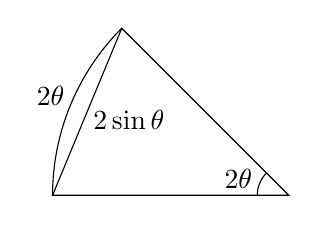
\begin{tikzpicture}
      \draw (-3, 0) -- (0, 0) -- (-2.121, 2.121) -- cycle node [pos=0.55, right] {$2 \sin \theta$};
      \draw (-3, 0) arc (180:135:3) node [pos=0.55, left] {$2 \theta$};

      \draw (-0.4, 0) arc(180:135:0.4) node [pos=0.7, left] {$2\theta$};
    \end{tikzpicture}
  \end{center}
  This means for $P, Q$ sufficiently close, we have $d(P, Q) \leq (1 + \varepsilon) |\overrightarrow{PQ}|$.

  From Analysis II, we know $\Gamma$ is uniformly continuous on $[0, 1]$. So we can choose $\mathcal{D}$ such that
  \[
    d(P_{i - 1}, P_i) \leq (1 + \varepsilon)|\overrightarrow{P_{i - 1}P_i}|
  \]
  for all $i$. So we know that for sufficiently fine $\mathcal{D}$,
  \[
    \tilde{S}_{\mathcal{D}} \leq (1 + \varepsilon) S_\mathcal{D} < d(P, Q),
  \]
  since $S_\mathcal{D} \to \ell$. However, by the triangle inequality $\tilde{S}_\mathcal{D} \geq d(P, Q)$. This is a contradiction. Hence we must have $\ell \geq d(P, Q)$.

  Suppose now $\ell = d(P, Q)$ for some $\Gamma: [0, 1] \to S$, $\ell = \length(\Gamma)$. Then for every $t \in [0, 1]$, we have
  \begin{align*}
    d(P, Q) = \ell &= \length \Gamma|_{[0, t]} + \length \Gamma|_{[t, 1]} \\
    &\geq d(P, \Gamma(t)) + d(\Gamma(t), Q)\\
    &\geq d(P, Q).
  \end{align*}
  Hence we must have equality all along the way, i.e.
  \[
    d(P, Q) = d(P, \Gamma(t)) + d(\Gamma(t), Q)
  \]
  for all $\Gamma(t)$.

  However, this is possible only if $\Gamma(t)$ lies on the shorter spherical line segment $PQ$, as we have previously proved. So done.
\end{proof}

Note that if $\Gamma$ is a curve of minimal length from $P$ to $Q$, then $\Gamma$ is a spherical line segment. Further, from the proof of this proposition, we know $\length \Gamma|_{[0, t]} = d(P, \Gamma(t))$ for all $t$. So the parametrisation of $\Gamma$ is monotonic. Such a $\Gamma$ is called a \emph{minimizing geodesic}.

Finally, we get to an important theorem whose prove involves complicated pictures. This is known as the \emph{Gauss-Bonnet theorem}. The Gauss-Bonnet theorem is in fact a much more general theorem. However, here we will specialize in the special case of the sphere. Later, when doing hyperbolic geometry, we will prove the hyperbolic version of the Gauss-Bonnet theorem. Near the end of the course, when we have developed sufficient machinery, we would be able to \emph{state} the Gauss-Bonnet theorem in its full glory. However, we will not be able to prove the general version.

\begin{prop}[Gauss-Bonnet theorem for $S^2$]
  If $\Delta$ is a spherical triangle with angles $\alpha, \beta, \gamma$, then
  \[
    \area (\Delta) = (\alpha + \beta + \gamma) - \pi.
  \]
\end{prop}

\begin{proof}
  \makeatletter
  \newcommand\filllunefront[9]{
    \pgfmathsetmacro{\x@x}{#3 * cos(#4)};
    \pgfmathsetmacro{\x@y}{#3 * sin(#4)};
    \pgfmathsetmacro{\y@x}{#3 * cos(#5)};
    \pgfmathsetmacro{\y@y}{#3 * sin(#5)};

    \color{#8};
    \pgfsetfillopacity{0.6};
    \pgfpathmoveto{\pgfpoint{#1}{#2}};
    \pgfpatharcto{#3 cm}{#6 cm}{#4}{0}{1}{\pgfpoint{-\x@x cm}{-\x@y cm}};
    \pgfpatharcto{#3 cm}{#3 cm}{0}{0}{#9}{\pgfpoint{-\y@x cm}{-\y@y cm}};
    \pgfpatharcto{#3 cm}{#7 cm}{#5}{0}{int(1-#9)}{\pgfpoint{#1}{#2}};
    \pgfusepath{fill};

    \pgfpathmoveto{\pgfpoint{#1}{#2}};
    \pgfpatharcto{#3 cm}{#6 cm}{#4}{0}{0}{\pgfpoint{\x@x cm}{\x@y cm}};
    \pgfpatharcto{#3 cm}{#3 cm}{0}{0}{#9}{\pgfpoint{\y@x cm}{\y@y cm}};
    \pgfpatharcto{#3 cm}{#7 cm}{#5}{0}{#9}{\pgfpoint{#1}{#2}};
    \pgfusepath{fill};
  }
  \newcommand\fillluneback[9]{
    \pgfmathsetmacro{\x@x}{#3 * cos(#4)};
    \pgfmathsetmacro{\x@y}{#3 * sin(#4)};
    \pgfmathsetmacro{\y@x}{#3 * cos(#5)};
    \pgfmathsetmacro{\y@y}{#3 * sin(#5)};

    \color{#8};

    \pgfsetfillopacity{0.11};
    \pgfpathmoveto{\pgfpoint{-#1}{-#2}};
    \pgfpatharcto{#3 cm}{#6 cm}{#4}{0}{0}{\pgfpoint{-\x@x cm}{-\x@y cm}};
    \pgfpatharcto{#3 cm}{#3 cm}{0}{0}{#9}{\pgfpoint{-\y@x cm}{-\y@y cm}};
    \pgfpatharcto{#3 cm}{#7 cm}{#5}{0}{#9}{\pgfpoint{-#1}{-#2}};
    \pgfusepath{fill};

    \pgfpathmoveto{\pgfpoint{-#1}{-#2}};
    \pgfpatharcto{#3 cm}{#6 cm}{#4}{0}{1}{\pgfpoint{\x@x cm}{\x@y cm}};
    \pgfpatharcto{#3 cm}{#3 cm}{0}{0}{#9}{\pgfpoint{\y@x cm}{\y@y cm}};
    \pgfpatharcto{#3 cm}{#7 cm}{#5}{0}{int(1-#9)}{\pgfpoint{-#1}{-#2}};
    \pgfusepath{fill};
  }
  \makeatother
  We start with the concept of a double lune. A \emph{double lune} with angle $0 < \alpha < \pi$ is two regions $S$ cut out by two planes through a pair of antipodal points, where $\alpha$ is the angle between the two planes.
  \begin{center}
    \begin{tikzpicture}
      \pgfdeclarelayer{col}
      \pgfsetlayers{col,main}
      \pgfmathsetmacro{\radius}{2.5}
      \pgfmathsetmacro{\ct}{20}
      \pgfmathsetmacro{\crad}{1.3}
      \pgfmathsetmacro{\dt}{70}
      \pgfmathsetmacro{\drad}{0.5}

      \draw circle [radius = \radius];

      \draw [name path=c1, rotate=\ct] (\radius, 0) arc(0:180:{\radius} and {\crad});
      \draw [opacity=0.6, name path=d1, rotate=\ct, dashed] (\radius, 0) arc(0:-180:{\radius} and {\crad});

      \draw [name path=c2, rotate=\dt] (\radius, 0) arc(0:180:{\radius} and {\drad});
      \draw [opacity=0.6, name path=d2, rotate=\dt, dashed] (\radius, 0) arc(0:-180:{\radius} and {\drad});

      \path [name intersections={of=c1 and c2,by=A}];
      \path [name intersections={of=d1 and d2,by=A'}];
      \node [circ] at (A) {};
      \node [circ] at (A') {};

      \node [anchor = south east] at (A) {$A$};
      \node [anchor = south east] at (A') {$A'$};

      \getCoord{\ax}{\ay}{A};
      \getCoord{\aax}{\aay}{A'};
      \begin{pgfonlayer}{col}
        \filllunefront{\ax}{\ay}{\radius}{\ct}{\dt}{\crad}{\drad}{mblue}{1};
        \fillluneback{\ax}{\ay}{\radius}{\ct}{\dt}{\crad}{\drad}{mblue}{1};
      \end{pgfonlayer}

    \end{tikzpicture}
  \end{center}
  It is not hard to show that the area of a double lune is $4 \alpha$, since the area of the sphere is $4\pi$.

  Now note that our triangle $\Delta = ABC$ is the intersection of 3 \emph{single} lunes, with each of $A, B, C$ as the pole (in fact we only need two, but it is more convenient to talk about $3$).
  \begin{center}
    \begin{tikzpicture}
      \pgfdeclarelayer{col}
      \pgfsetlayers{col,main}
      \pgfmathsetmacro{\radius}{2.5}
      \pgfmathsetmacro{\ct}{20}
      \pgfmathsetmacro{\crad}{1.3}
      \pgfmathsetmacro{\dt}{70}
      \pgfmathsetmacro{\drad}{0.5}
      \pgfmathsetmacro{\et}{140}
      \pgfmathsetmacro{\erad}{0.5}

      \draw circle [radius = \radius];

      \draw [name path=c1, rotate=\ct] (\radius, 0) arc(0:180:{\radius} and {\crad});
      \draw [opacity=0.6, name path=c2, rotate=\ct, dashed] (\radius, 0) arc(0:-180:{\radius} and {\crad});

      \draw [name path=d1, rotate=\dt] (\radius, 0) arc(0:180:{\radius} and {\drad});
      \draw [opacity=0.6, name path=d2, rotate=\dt, dashed] (\radius, 0) arc(0:-180:{\radius} and {\drad});

      \draw [name path=e1, rotate=\et] (\radius, 0) arc(0:180:{\radius} and {\erad});
      \draw [opacity=0.6, name path=e2, rotate=\et, dashed] (\radius, 0) arc(0:-180:{\radius} and {\erad});

      \path [name intersections={of=c1 and d1,by=A}];
      \path [name intersections={of=c2 and d2,by=A'}];
      \node [circ] at (A) {};
      \node [opacity=0.6, circ] at (A') {};
      \node [anchor = south east] at (A) {$A$};
      \node [opacity=0.6, anchor = south east] at (A') {$A'$};

      \path [name intersections={of=c1 and e1,by=B}];
      \path [name intersections={of=c2 and e2,by=B'}];
      \node [circ] at (B) {};
      \node [opacity=0.6, circ] at (B') {};
      \node [left] at (B) {$B$};
      \node [opacity=0.6, right] at (B') {$B'$};

      \path [name intersections={of=d1 and e1,by=C}];
      \path [name intersections={of=d2 and e2,by=C'}];
      \node [circ] at (C) {};
      \node [opacity=0.6, circ] at (C') {};
      \node [right] at (C) {$C$};
      \node [opacity=0.6, right] at (C') {$C'$};

      \getCoord{\ax}{\ay}{A};
      \getCoord{\bx}{\by}{B};
      \getCoord{\cx}{\cy}{C};

      \begin{pgfonlayer}{col}
        \fillluneback{\ax}{\ay}{\radius}{\ct}{\dt}{\crad}{\drad}{mblue}{1};
        \fillluneback{\bx}{\by}{\radius}{\ct}{180+\et}{\crad}{\erad}{mgreen}{0};
        \fillluneback{\cx}{\cy}{\radius}{\dt}{\et}{\drad}{\erad}{morange}{1};

        \filllunefront{\ax}{\ay}{\radius}{\ct}{\dt}{\crad}{\drad}{mblue}{1};
        \filllunefront{\bx}{\by}{\radius}{\ct}{180+\et}{\crad}{\erad}{mgreen}{0};
        \filllunefront{\cx}{\cy}{\radius}{\dt}{\et}{\drad}{\erad}{morange}{1};
      \end{pgfonlayer}
    \end{tikzpicture}
  \end{center}
  Therefore $\Delta$ together with its antipodal partner $\Delta'$ is a subset of each of the 3 double lunes with areas $4\alpha, 4\beta, 4\gamma$. Also, the union of all the double lunes cover the whole sphere, and overlap at exactly $\Delta$ and $\Delta'$.
  Thus
  \[
    4(\alpha + \beta + \gamma) = 4\pi + 2(\area(\Delta) + \area(\Delta')) = 4\pi + 4 \area(\Delta).\qedhere
  \]
\end{proof}
This is easily generalized to arbitrary convex $n$-gons on $S^2$ (with $n \geq 3$). Suppose $M$ is such a convex $n$-gon with interior angles $\alpha_1, \cdots, \alpha_n$. Then we have
\[
  \area(M) = \sum_1^n \alpha_i - (n - 2) \pi.
\]
This follows directly from cutting the polygon up into the constituent triangles.

This is very unlike Euclidean space. On $\R^2$, we always have $\alpha + \beta + \gamma = \pi$. Not only is this false on $S^2$, but by measuring the difference, we can tell the area of the triangle. In fact, we can identify triangles up to congruence just by knowing the three angles.

\subsection{M\texorpdfstring{\"o}{o}bius geometry}
It turns out it is convenient to identify the sphere $S^2$ withe the extended complex plane $\C_\infty = \C \cup \{\infty\}$. Then isometries of $S^2$ will translate to nice class of maps of $\C_\infty$.

We first find a way to identify $S^2$ with $C_\infty$. We use coordinates $\zeta \in \C_\infty$. We define the \emph{stereographic projection} $\pi: S^2 \to \C_\infty$ by
\begin{center}
  \begin{tikzpicture}
    \draw (0, 0) -- (8, 0) -- (10, 3) -- (2, 3) -- (0, 0);
    \draw [gray] (1, 1.5) -- (9, 1.5);
    \draw [gray] (4, 0) -- (6, 3);
    \draw (6.2, 1.5) arc(0:180:1.2);
    \draw [opacity=0.5] (6.2, 1.5) arc(0:-180:1.2);
    \draw (6.2, 1.5) arc(0:-180:1.2 and 0.5);
    \draw [dashed] (6.2, 1.5) arc(0:180:1.2 and 0.5);

    \node [circ] at (5, 2.5) {};
    \node at (5, 2.5) [right] {$N$};

    \node [circ] at (5.5, 2.17) {};
    \node at (5.5, 2.17) [right] {$P$};

    \draw (5, 2.5) -- (7, 1.2) node [circ] {} node [right] {$\pi(P)$};
  \end{tikzpicture}
\end{center}
\[
  \pi(P) = (\text{line } PN)\cap \{z = 0\},
\]
which is well defined except where $P = N$, in which case we define $\pi(N) = \infty$.

To give an explicit formula for this, consider the cross-section through the plane $ONP$.
\begin{center}
  \begin{tikzpicture}
    \node [circ] {};
    \node [anchor = north east] {$O$};
    \draw circle [radius=2];
    \draw (-3, 0) -- (5.5, 0);
    \draw (0, 0) -- (0, 2) node [circ] {} node [above] {$N$};
    \draw (0, 1.414) -- (1.414, 1.414) node [pos=0.5, below] {$r$} node [right] {$P$} node [circ] {};
    \draw (0.2, 1.414) -- +(0, 0.2) -- +(-0.2, 0.2);

    \draw [<->] (-0.245, 0) -- +(0, 1.414) node [fill=white, pos=0.5] {$z$};
    \draw (0, 2) -- (4.8259, 0) node [circ] {} node [above] {$\pi(P)$};

    \draw [<->] (0, -0.245) -- +(4.8259, 0) node [fill=white, pos=0.5] {$R$};
  \end{tikzpicture}
\end{center}
If $P$ has coordinates $(x, y)$, then we see that $\pi(P)$ will be a scalar multiple of $x + iy$. To find this factor, we notice that we have two similar triangles, and hence obtain
\[
  \frac{r}{R} = \frac{1 - z}{1}.
\]
Then we obtain the formula
\[
  \pi(x, y, z) = \frac{x + iy}{1 - z}.
\]
If we do the projection from the South pole instead, we get a related formula.
\begin{lemma}
  If $\pi': S^2 \to \C_{\infty}$ denotes the stereographic projection from the South Pole instead, then
  \[
    \pi'(P) = \frac{1}{\overline{\pi(P)}}.
  \]
\end{lemma}

\begin{proof}
  Let $P(x, y, z)$. Then
  \[
    \pi(x, y, z) = \frac{x + iy}{1 - z}.
  \]
  Then we have
  \[
    \pi'(x, y, z) = \frac{x + iy}{1 + z},
  \]
  since we have just flipped the $z$ axis around. So we have
  \[
    \overline{\pi(P)}\pi'(P) = \frac{x^2 + y^2}{1 - z^2} =1,
  \]
  noting that we have $x^2 + y^2 + z^2 = 1$ since we are on the unit sphere.
\end{proof}

We can use this to infer that $\pi' \circ \pi^{-1}: C_{\infty} \to C_{\infty}$ takes $\zeta \mapsto 1/\bar{\zeta}$, which is the inversion in the unit circle $|\zeta| = 1$.

From IA Groups, we know M\"obius transformations act on $\C_{\infty}$ and form a group $G$ by composition. For each matrix
\[
  A =
  \begin{pmatrix}
    a & b\\
    c & d
  \end{pmatrix} \in \GL(2, \C),
\]
we get a M\"obius map $\C_\infty \to \C_\infty$ by
\[
  \zeta \mapsto \frac{a \zeta + b}{c \zeta + d}.
\]
Moreover, composition of M\"obius map is the same multiplication of matrices.

This is not exactly a bijective map between $G$ and $\GL(2, \C)$. For any $\lambda \in \C^* = \C \setminus \{0\}$, we know $\lambda A$ defines the same map M\"obius map as $A$. Conversely, if $A_1$ and $A_2$ gives the same M\"obius map, then there is some $\lambda_1 \not= 0$ such that $A_1 = \lambda A_2$.

Hence, we have
\[
  G \cong \PGL(2, \C) = \GL(2, \C)/\C^*,
\]
where
\[
  \C^* \cong \{ \lambda I: \lambda \in \C^*\}.
\]
Instead of taking the whole $\GL(2, \C)$ and quotienting out multiples of the identities, we can instead start with $\SL(2, \C)$. Again, $A_1, A_2 \in \SL(2, \C)$ define the same map if and only if $A_1 = \lambda A_2$ for some $\lambda$. What are the possible values of $\lambda$? By definition of the special linear group, we must have
\[
  1 = \det(\lambda A) = \lambda^2 \det A = \lambda^2.
\]
So $\lambda^2 = \pm 1$. So each M\"obius map is represented by two matrices, $A$ and $-A$, and we get
\[
  G \cong \PSL(2, \C) = \SL(2, \C)/\{\pm 1\}.
\]
Now let's think about the sphere. On $S^2$, the rotations $\SO(3)$ act as isometries. In fact, the full isometry group of $S^2$ is $\Or(3)$ (the proof is on the first example sheet). What we would like to show that rotations of $S^2$ correspond to M\"obius transformations coming from the subgroup $\SU(2) \leq \GL(2, \C)$.

\begin{thm}
  Via the stereographic projection, every rotation of $S^2$ induces a M\"obius map defined by a matrix in $\SU(2) \subseteq \GL(2, \C)$, where
  \[
    \SU(2) = \left\{
      \begin{pmatrix}
        a & -b\\
        \bar{b} & \bar{a}
      \end{pmatrix}
      : |a|^2 + |b|^2 = 1
    \right\}.
  \]
\end{thm}

\begin{proof}\leavevmode
  \begin{enumerate}
    \item Consider the $r(\hat{\mathbf{z}}, \theta)$, the rotations about the $z$ axis by $\theta$. These corresponds to the M\"obius map $\zeta \mapsto e^{i\theta} \zeta$, which is given by the unitary matrix
      \[
        \begin{pmatrix}
          e^{i\theta/2} & 0\\
          0 & e^{-i\theta/2}.
        \end{pmatrix}
      \]
    \item Consider the rotation $r(\hat{\mathbf{y}}, \frac{\pi}{2})$. This has the matrix
      \[
        \begin{pmatrix}
          0 & 0 & 1\\
          0 & 1 & 0\\
          -1 & 0 & 0
        \end{pmatrix}
        \begin{pmatrix}
          x\\y\\z
        \end{pmatrix}
        =
        \begin{pmatrix}
          z\\y\\-x
        \end{pmatrix}.
      \]
      This corresponds to the map
      \[
        \zeta = \frac{x + iy}{1 - z} \mapsto \zeta' = \frac{z + iy}{1 + x}
      \]
      We want to show this is a M\"obius map. To do so, we guess what the M\"obius map should be, and check it works. We can manually compute that $-1 \mapsto \infty$, $1 \mapsto 0$, $i \mapsto i$.
      \begin{center}
        \begin{tikzpicture}
          \draw circle [radius=2.5];
          \draw (-2.5, 0) arc(180:360:2.5 and 0.5);
          \draw [dashed] (-2.5, 0) arc(180:0:2.5 and 0.6);

          \node [circ] at (-2.5, 0) {};
          \node [circ] at (2.5, 0) {};
          \node [circ] at (-0.5, -0.49) {};
          \node [left] at (-2.5, 0) {$1$};
          \node [right] at (2.5, 0) {$-1$};
          \node [below] at (-0.5, -0.49) {$i$};

          \node [circ] at (0, -2.5) {};
          \node [below] at (0, -2.5) {$0$};
          \node [circ] at (0, 2.5) {};
          \node [above] at (0, 2.5) {$\infty$};
        \end{tikzpicture}
      \end{center}
      The only M\"obius map that does this is
      \[
        \zeta' = \frac{\zeta - 1}{\zeta + 1}.
      \]
      We now check:
      \begin{align*}
        \frac{\zeta - 1}{\zeta + 1} &= \frac{x + iy - 1 + z}{x + iy + 1 - z}\\
        &= \frac{x - 1 + z + iy}{x + 1 - (z - iy)}\\
        &= \frac{(z + iy)(x - 1 + z + iy)}{(x + 1)(z + iy) - (z^2 + y^2)}\\
        &= \frac{(z + iy)(x - 1 + z + iy)}{(x + 1)(z + iy) + (x^2 - 1)}\\
        &= \frac{(z + iy)(x - 1 + z + iy)}{(x + 1)(z + iy + x - 1)}\\
        &= \frac{z + iy}{x + 1}.
      \end{align*}
      So done. We finally have to write this in the form of an $\SU(2)$ matrix:
      \[
        \frac{1}{\sqrt{2}}
        \begin{pmatrix}
          1 & -1\\
          1 & 1
        \end{pmatrix}.
      \]
    \item We claim that $\SO(3)$ is generated by $r\left(\hat{\mathbf{y}}, \frac{\pi}{2}\right)$ and $r(\hat{\mathbf{z}}, \theta)$ for $0 \leq \theta < 2\pi$.

      To show this, we observe that $r(\hat{\mathbf{x}}, \varphi) = r(\hat{\mathbf{y}}, \frac{\pi}{2}) r(\hat{\mathbf{z}}, \varphi) r(\hat{\mathbf{y}}, -\frac{\pi}{2})$. Note that we read the composition from right to left. You can convince yourself this is true by taking a physical sphere and try rotating. To prove it formally, we can just multiply the matrices out.

      Next, observe that for $\mathbf{v} \in S^2 \subseteq \R^3$, there are some angles $\varphi, \psi$ such that $g = r(\hat{\mathbf{z}}, \psi) r(\hat{\mathbf{x}}, \varphi)$ maps $\mathbf{v}$ to $\hat{\mathbf{x}}$. We can do so by first picking $r(\hat{\mathbf{x}}, \varphi)$ to rotate $\mathbf{v}$ into the $(x, y)$-plane. Then we rotate about the $z$-axis to send it to $\hat{\mathbf{x}}$.

      Then for any $\theta$, we have $r(\mathbf{v}, \theta) = g^{-1} r(\hat{\mathbf{x}}, \theta) g$, and our claim follows by composition.
    \item Thus, via the stereographic projection, every rotation of $S^2$ corresponds to products of M\"obius transformations of $\C_\infty$ with matrices in $\SU(2)$.\qedhere
  \end{enumerate}
\end{proof}
The key of the proof is step (iii). Apart from enabling us to perform the proof, it exemplifies a useful technique in geometry --- we know how to rotate arbitrary things in the $z$ axis. When we want to rotate things about the $x$ axis instead, we first rotate the sphere to move the $x$ axis to where the $z$ axis used to be, do those rotations, and then rotate it back. In general, we can use some isometries or rotations to move what we want to do to a convenient location.

\begin{thm}
  The group of rotations $\SO(3)$ acting on $S^2$ corresponds precisely with the subgroup $\PSU(2) = \SU(2)/ \pm 1$ of M\"obius transformations acting on $\C_\infty$.
\end{thm}
What this is in some sense a converse of the previous theorem. We are saying that for each M\"obius map from $\SU(2)$, we can find some rotation of $S^2$ that induces that M\"obius map, and there is exactly one.

\begin{proof}
  Let $g \in \PSU(2)$ be a M\"obius transformation
  \[
    g(z) = \frac{az + b}{\bar{b} z + \bar{a}}.
  \]
  Suppose first that $g(0) = 0$. So $b = 0$. So $a\bar{a} = 1$. Hence $a = e^{i\theta/2}$. Then $g$ corresponds to $r(\hat{\mathbf{z}}, \theta)$, as we have previously seen.

  In general, let $g(0) = w \in \C_\infty$. Let $Q \in S^2$ be such that $\pi(Q) = w$. Choose a rotation $A \in \SO(3)$ such that $A(Q) = -\hat{\mathbf{z}}$. Since $A$ is a rotation, let $\alpha \in \PSU(2)$ be the corresponding M\"obius transformation. By construction we have $\alpha(w) = 0$. Then the composition $\alpha \circ g$ fixes zero. So it corresponds to some $B = r(z, \theta)$. We then see that $g$ corresponds to $A^{-1} B \in \SO(3)$. So done.
\end{proof}
Again, we solved an easy case, where $g(0) = 0$, and then performed some rotations to transform any other case into this simple case.

We have now produced a $2$-to-$1$ map
\[
  \SU(2) \to \PSU(2) \cong \SO(3).
\]
If we treat these groups as topological spaces, this map does something funny.

Suppose we start with a (non-closed) path from $I$ to $-I$ in $\SU(2)$. Applying the map, we get a \emph{closed} loop from $I$ to $I$ in $\SO(3)$.

Hence, in $\SO(3)$, loops are behave slightly weirdly. If we go around this loop in $\SO(3)$, we didn't really get back to the same place. Instead, we have actually moved from $I$ to $-I$ in $\SU(2)$. It takes \emph{two} full loops to actually get back to $I$. In physics, this corresponds to the idea of spinors.

We can also understand this topologically as follows: since $\SU(2)$ is defined by two complex points $a, b \in \C$ such that $|a|^2 + |b|^2$, we can view it as as three-sphere $S^3$ in $\SO(3)$.

A nice property of $S^3$ is it is \emph{simply connected}, as in any loop in $S^3$ can be shrunk to a point. In other words, given any loop in $S^3$, we can pull and stretch it (continuously) until becomes the ``loop'' that just stays at a single point.

On the other hand, $\SO(3)$ is not simply connected. We have just constructed a loop in $\SO(3)$ by mapping the path from $I$ to $-I$ in $\SU(2)$. We \emph{cannot} deform this loop until it just sits at a single point, since if we lift it back up to $\SU(2)$, it still has to move from $I$ to $-I$.

The neat thing is that in some sense, $S^3 \cong \SU(2)$ is just ``two copies'' of $\SO(3)$. By duplicating $\SO(3)$, we have produced $\SU(2)$, a simply connected space. Thus we say $\SU(2)$ is a \emph{universal cover} of $\SO(3)$.

We've just been waffling about spaces and loops, and throwing around terms we haven't defined properly. These vague notions will be made precise in the IID Algebraic Topology course, and we will then (maybe) see that $\SU(2)$ is a \emph{universal cover} of $\SO(3)$.

\section{Triangulations and the Euler number}
We shall now study the idea of triangulations and the Euler number. We aren't going to do much with them in this course --- we will not even prove that the Euler number is a well-defined number. However, we need Euler numbers in order to state the full Gauss-Bonnet theorem at the end, and the idea of triangulations is useful in the IID Algebraic Topology course for defining simplicial homology. More importantly, the discussion of these concepts is required by the schedules. Hence we will get \emph{some} exposure to these concepts in this chapter.

It is convenient to have an example other than the sphere when discussing triangulations and Euler numbers. So we introduce the \emph{torus}
\begin{defi}[(Euclidean) torus]
  The \emph{(Euclidean) torus} is the set $\R^2/\Z^2$ of equivalence classes of $(x, y) \in \R^2$ under the equivalence relation
  \[
    (x_1, y_1) \sim (x_2, y_2) \Leftrightarrow x_1 - x_2, y_1 - y_2 \in \Z.
  \]
\end{defi}
It is easy to see this is indeed an equivalence relation. Thus a point in $T$ represented by $(x, y)$ is a coset $(x, y) + \Z^2$ of the subgroup $\Z^2 \leq \R^2$.

Of course, there are many ways to represent a point in the torus. However, for any closed square $Q \subseteq \R^2$ with side length $1$, we can obtain $T$ is by identifying the sides
\begin{center}
  \begin{tikzpicture}
    \draw [mred, ->-=0.58] (0, 0) -- +(2, 0);
    \draw [mred, ->-=0.58] (0, 2) -- +(2, 0);

    \draw [mblue, ->>-=0.63] (0, 0) -- +(0, 2);
    \draw [mblue, ->>-=0.63] (2, 0) -- +(0, 2);

    \node at (1, 1) {$Q$};
  \end{tikzpicture}
\end{center}
We can define a distance $d$ for all $P_1, P_2 \in T$ to be
\[
  d(P_1, P_2) = \min\{\|\mathbf{v}_1 - \mathbf{v}_2\|: \mathbf{v}_i \in \R^2, \mathbf{v}_i + \Z^2 = P_i\}.
\]
It is not hard to show this definition makes $(T, d)$ into a metric space. This allows us to talk about things like open sets and continuous functions. We will later show that this is not just a metric space, but a \emph{smooth surface}, after we have defined what that means.

We write $\mathring{Q}$ for the interior of $Q$. Then the natural map $f: \mathring{Q} \to T$ given by $\mathbf{v} \mapsto \mathbf{v} + \Z^2$ is a bijection onto some open set $U \subseteq T$. In fact, $U$ is just $T \setminus \{\text{two circles meeting in 1 point}\}$, where the two circles are the boundary of the square $Q$.

Now given any point in the torus represented by $P + \Z^2$, we can find a square $Q$ such that $P \in \mathring{Q}$. Then $f: \mathring{Q} \to T$ restricted to an open disk about $P$ is an isometry (onto the image, a subset of $\R^2$). Thus we say $d$ is a \emph{locally Euclidean metric}.

One can also think of the torus $T$ as the surface of a doughnut, ``embedded'' in Euclidean space $\R^3$.
\begin{center}
  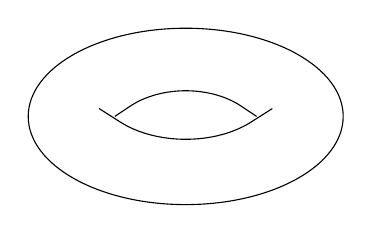
\begin{tikzpicture}
    \draw (0,0) ellipse (2 and 1.12);
    \path[rounded corners=24pt] (-.9,0)--(0,.6)--(.9,0) (-.9,0)--(0,-.56)--(.9,0);
    \draw[rounded corners=28pt] (-1.1,.1)--(0,-.6)--(1.1,.1);
    \draw[rounded corners=24pt] (-.9,0)--(0,.6)--(.9,0);
  \end{tikzpicture}
\end{center}
Given this, it is natural to define the distance between two points to be the length of the shortest curve between them on the torus. However, this distance function is \emph{not} the same as what we have here. So it is misleading to think of our locally Euclidean torus as a ``doughnut''.

With one more example in our toolkit, we can start doing what we really want to do. The idea of a triangulation is to cut a space $X$ up into many smaller triangles, since we like triangles. However, we would like to first define what a triangle is.
\begin{defi}[Topological triangle]
  A \emph{topological triangle} on $X = S^2$ or $T$ (or any metric space $X$) is a subset $R \subseteq X$ equipped with a homeomorphism $R \to \Delta$, where $\Delta$ is a closed Euclidean triangle in $\R^2$.
\end{defi}
Note that a spherical triangle is in fact a topological triangle, using the radial projection to the plane $\R^2$ from the center of the sphere.
\begin{defi}[Topological triangulation]
  A \emph{topological triangulation} $\tau$ of a metric space $X$ is a finite collection of topological triangles of $X$ which cover $X$ such that
  \begin{enumerate}
    \item For every pair of triangles in $\tau$, either they are disjoint, or they meet in exactly one edge, or meet at exactly one vertex.
    \item Each edge belongs to exactly two triangles.
  \end{enumerate}
\end{defi}
These notions are useful only if the space $X$ is ``two dimensional'' --- there is no way we can triangulate, say $\R^3$, or a line. We can generalize triangulation to allow higher dimensional ``triangles'', namely topological tetrahedrons, and in general, $n$-simplices, and make an analogous definition of triangulation. However, we will not bother ourselves with this.

\begin{defi}[Euler number]
  The \emph{Euler number} of a triangulation $e = e(X, \tau)$ is
  \[
    e = F - E + V,
  \]
  where $F$ is the number of triangles; $E$ is the number of edges; and $V$ is the number of vertices.
\end{defi}
Note that each edge actually belongs to two triangles, but we will only count it once.

There is one important fact about triangulations from algebraic topology, which we will state without proof.
\begin{thm}
  The Euler number $e$ is independent of the choice of triangulation.
\end{thm}
So the Euler number $e = e(X)$ is a property of the space $X$ itself, not a particular triangulation.

\begin{eg}
  Consider the following triangulation of the sphere:
  \begin{center}
    \begin{tikzpicture}
      \draw circle [radius=2];
      \draw [name path=eqf] (-2, 0) arc(180:360:2 and 0.5);
      \draw [dashed, name path=eqb] (-2, 0) arc(180:0:2 and 0.5);
      \draw [name path=verf] (0, 2) arc(90:270:0.5 and 2);
      \draw [dashed, name path=verb] (0, 2) arc(90:-90:0.5 and 2);
      \node [circ] at (2, 0) {};
      \node [circ] at (0, 2) {};
      \node [circ] at (-2, 0) {};
      \node [circ] at (0, -2) {};

      \path [name intersections={of=eqf and verf,by=F}];
      \node [circ] at (F) {};
      \path [name intersections={of=eqb and verb,by=B}];
      \node [circ] at (B) {};
    \end{tikzpicture}
  \end{center}
  This has $8$ faces, $12$ edges and $6$ vertices. So $e = 2$.
\end{eg}

\begin{eg}
  Consider the following triangulation of the torus. Be careful not to double count the edges and vertices at the sides, since the sides are glued together.
  \begin{center}
    \begin{tikzpicture}
      \draw [mred, ->-=0.55] (0, 0) -- +(3, 0);
      \draw [mred, ->-=0.55] (0, 3) -- +(3, 0);

      \draw [mblue, ->>-=0.6] (0, 0) -- +(0, 3);
      \draw [mblue, ->>-=0.6] (3, 0) -- +(0, 3);
      \foreach \x in {1,2} {
        \draw (\x, 0) -- +(0, 3);
        \draw (0, \x) -- +(3, 0);
      }
      \draw (0, 0) -- (3, 3);
      \draw (1, 0) -- (3, 2);
      \draw (2, 0) -- (3, 1);
      \draw (0, 1) -- (2, 3);
      \draw (0, 2) -- (1, 3);
    \end{tikzpicture}
  \end{center}
  This has $18$ faces, $27$ edges and $9$ vertices. So $e = 0$.
\end{eg}
In both cases, we did not cut up our space with funny, squiggly lines. Instead, we used ``straight'' lines. These triangles are known as \emph{geodesic triangles}.

\begin{defi}[Geodesic triangle]
  A \emph{geodesic triangle} is a triangle whose sides are geodesics, i.e.\ paths of shortest distance between two points.
\end{defi}
In particular, we used spherical triangles in $S^2$ and Euclidean triangles in $\mathring{Q}$. Triangulations made of geodesic triangles are rather nice. They are so nice that we can actually prove something about them!
\begin{prop}
  For every geodesic triangulation of $S^2$ (and respectively $T$) has $e = 2$ (respectively, $e = 0$).
\end{prop}
Of course, we know this is true for \emph{any} triangulation, but it is difficult to prove that without algebraic topology.

\begin{proof}
  For any triangulation $\tau$, we denote the ``faces'' of $\Delta_1, \cdots, \Delta_F$, and write $\tau_i = \alpha_i + \beta_i + \gamma_i$ for the sum of the interior angles of the triangles (with $i = 1, \cdots, F$).

  Then we have
  \[
    \sum \tau_i = 2 \pi V,
  \]
  since the total angle around each vertex is $2\pi$. Also, each triangle has three edges, and each edge is from two triangles. So $3F = 2E$. We write this in a more convenient form:
  \[
    F = 2E - 2F.
  \]
  How we continue depends on whether we are on the sphere or the torus.
  \begin{itemize}
    \item For the sphere, Gauss-Bonnet for the sphere says the area of $\Delta_i$ is $\tau_i - \pi$. Since the area of the sphere is $4\pi$, we know
      \begin{align*}
        4\pi &= \sum \area(\Delta_i) \\
        &= \sum (\tau_i - \pi) \\
        &= 2\pi V - F\pi \\
        &= 2\pi V - (2E - 2F)\pi \\
        &= 2\pi (F - E + V).
      \end{align*}
      So $F - E + V = 2$.
    \item For the torus, we have $\tau_i = \pi$ for every face in $\mathring{Q}$. So
      \[
        2\pi V = \sum \tau_i = \pi F.
      \]
      So
      \[
        2V = F = 2E - 2F.
      \]
      So we get
      \[
        2(F - V + E) = 0,
      \]
      as required.\qedhere
  \end{itemize}
\end{proof}
Note that in the definition of triangulation, we decomposed $X$ into topological triangles. We can also use decompositions by topological polygons, but they are slightly more complicated, since we have to worry about convexity. However, apart from this, everything works out well. In particular, the previous proposition also holds, and we have Euler's formula for $S^2$: $V - E + F = 2$ for any polygonal decomposition of $S^2$. This is not hard to prove, and is left as an exercise on the example sheet.

\section{Hyperbolic geometry}
At the beginning of the course, we studied Euclidean geometry, which was not hard, because we already knew about it. Later on, we studied spherical geometry. That also wasn't too bad, because we can think of $S^2$ concretely as a subset of $\R^3$.

We are next going to study hyperbolic geometry. Historically, hyperbolic geometry was created when people tried to prove Euclid's parallel postulate (that given a line $\ell$ and a point $P \not\in \ell$, there exists a unique line $\ell'$ containing $P$ that does not intersect $\ell$). Instead of proving the parallel postulate, they managed to create a new geometry where this is false, and this is hyperbolic geometry.

Unfortunately, hyperbolic geometry is much more complicated, since we cannot directly visualize it as a subset of $\R^3$. Instead, we need to develop the machinery of a \emph{Riemannian metric} in order to properly describe hyperbolic geometry. In a nutshell, this allows us to take a subset of $\R^2$ and measure distances in it in a funny way.

\subsection{Review of derivatives and chain rule}
We start by reviewing some facts about taking derivatives, and make explicit the notation we will use.

\begin{defi}[Smooth function]
  Let $U \subseteq \R^n$ be open, and $f = (f_1, \cdots, f_m): U \to \R^m$. We say $f$ is \emph{smooth} (or $C^\infty$) if each $f_i$ has continuous partial derivatives of each order. In particular, a $C^\infty$ map is differentiable, with continuous first-order partial derivatives.
\end{defi}

\begin{defi}[Derivative]
  The \emph{derivative} for a function $f: U \to \R^m$ at a point $a \in U$ is a linear map $\d f_a: \R^n \to \R^m$ (also written as $\D f(a)$ or $f'(a)$) such that
  \[
    \lim_{h \to 0} \frac{\|f(a + h) - f(a) - \d f_a \cdot h\|}{\|h\|} \to 0,
  \]
  where $h \in \R^n$.

  If $m = 1$, then $\d f_a$ is expressed as $\left(\frac{\partial f}{\partial x_a}(a), \cdots, \frac{\partial f}{\partial x_n}(a)\right)$, and the linear map is given by
  \[
    (h_1, \cdots, h_n) \mapsto \sum_{i = 1}^n \frac{\partial f}{\partial x_i}(a) h_i,
  \]
  i.e.\ the dot product. For a general $m$, this vector becomes a matrix. The \emph{Jacobian matrix} is
  \[
    J(f)_a = \left(\frac{\partial f_i}{\partial x_j}(a)\right),
  \]
  with the linear map given by matrix multiplication, namely
  \[
    h \mapsto J(f)_a \cdot h.
  \]
\end{defi}

\begin{eg}
  Recall that a holomorphic (analytic) function of complex variables $f: U \subseteq \C \to \C$ has a derivative $f'$, defined by
  \[
    \lim_{|w| \to 0} \frac{|f(z + w) - f(z) - f'(z) w|}{|w|} \to 0
  \]
  We let $f'(z) = a + ib$ and $w = h_1 + i h_2$. Then we have
  \[
    f'(z) w = ah_1 - bh_2 + i(ah_2 + bh_1).
  \]
  We identify $\R^2 = \C$. Then $f: U \subseteq \R^2 \to \R^2$ has a derivative $\d f_z: \R^2 \to \R^2$ given by
  \[
    \begin{pmatrix}
      a & -b\\
      b & a
    \end{pmatrix}.
  \]
\end{eg}

We're also going to use the chain rule quite a lot. So we shall write it out explicitly.
\begin{prop}[Chain rule]
  Let $U \subseteq \R^n$ and $V\subseteq \R^p$. Let $f: U \to \R^m$ and $g: V \to U$ be smooth. Then $f \circ g: V \to \R^m$ is smooth and has a derivative
  \[
    d(f \circ g)_p = (\d f)_{g(p)} \circ (\d g)_p.
  \]
  In terms of the Jacobian matrices, we get
  \[
    J(f \circ g)_p = J(f)_{g(p)}J(g)_p.
  \]
\end{prop}

\subsection{Riemannian metrics}
Finally, we get to the idea of a Riemannian metric. The basic idea of a Riemannian metric is not too unfamiliar. Presumably, we have all seen maps of the Earth, where we try to draw the spherical Earth on a piece of paper, i.e.\ a subset of $\R^2$. However, this does not behave like $\R^2$. You cannot measure distances on Earth by placing a ruler on the map, since distances are distorted. Instead, you have to find the coordinates of the points (e.g.\ the longitude and latitude), and then plug them into some complicated formula. Similarly, straight lines on the map are not really straight (spherical) lines on Earth.

We really should not think of Earth a subset of $\R^2$. All we have done was to ``force'' Earth to live in $\R^2$ to get a convenient way of depicting the Earth, as well as a convenient system of labelling points (in many map projections, the $x$ and $y$ axes are the longitude and latitude).

This is the idea of a Riemannian metric. To describe some complicated surface, we take a subset $U$ of $\R^2$, and define a new way of measuring distances, angles and areas on $U$. All these information are packed into an entity known as the \emph{Riemannian metric}.

\begin{defi}[Riemannian metric]
  We use coordinates $(u, v) \in \R^2$. We let $V \subseteq \R^2$ be open. Then a Riemannian metric on $V$ is defined by giving $C^{\infty}$ functions $E, F, G: V \to \R$ such that
  \[
    \begin{pmatrix}
      E(P) & F(P)\\
      F(P) & G(P)
    \end{pmatrix}
  \]
  is a positive definite definite matrix for all $P \in V$.

  Alternatively, this is a smooth function that gives a $2\times 2$ symmetric positive definite matrix, i.e.\ inner product $\bra \ph, \ph\ket_P$, for each point in $V$. By definition, if $\mathbf{e}_1, \mathbf{e}_2$ are the standard basis, then
  \begin{align*}
    \bra \mathbf{e}_1, \mathbf{e}_1\ket_P &= E(P)\\
    \bra \mathbf{e}_1, \mathbf{e}_2\ket_P &= F(P)\\
    \bra \mathbf{e}_2, \mathbf{e}_2\ket_P &= G(P).
  \end{align*}
\end{defi}
\begin{eg}
  We can pick $E = G = 1$ and $F = 0$. Then this is just the standard Euclidean inner product.
\end{eg}

As mentioned, we should not imagine $V$ as a subset of $\R^2$. Instead, we should think of it as an abstract two-dimensional surface, with some coordinate system given by a subset of $\R^2$. However, this coordinate system is just a convenient way of labelling points. They do not represent any notion of distance. For example, $(0, 1)$ need not be closer to $(0, 2)$ than to $(7, 0)$. These are just abstract labels.

With this in mind, $V$ does not have any intrinsic notion of distances, angles and areas. However, we do want these notions. We can certainly \emph{write down} things like the difference of two points, or even the compute the derivative of a function. However, these numbers you get are not meaningful, since we can easily use a different coordinate system (e.g.\ by scaling the axes) and get a different number. They have to be interpreted with the \emph{Riemannian metric}. This tells us how to measure these things, via an inner product ``that varies with space''. This variation in space is not an oddity arising from us not being able to make up our minds. This is since we have ``forced'' our space to lie in $\R^2$. Inside $V$, going from $(0, 1)$ to $(0, 2)$ might be very different from going from $(5, 5)$ to $(6, 5)$, since coordinates don't mean anything. Hence our inner product needs to measure ``going from $(0, 1)$ to $(0, 2)$'' differently from ``going from $(5, 5)$ to $(6, 5)$'', and must vary with space.

We'll soon come to defining how this inner product gives rise to the notion of distance and similar stuff. Before that, we want to understand what we can put into the inner product $\bra\ph, \ph\ket_P$. Obviously these would be vectors in $\R^2$, but where do these vectors come from? What are they supposed to represent?

The answer is ``directions'' (more formally, tangent vectors). For example, $\bra \mathbf{e}_1, \mathbf{e}_1\ket_P$ will tell us how far we actually are going if we move in the direction of $\mathbf{e}_1$ from $P$. Note that we say ``move in the direction of $\mathbf{e}_1$'', not ``move by $\mathbf{e}_1$''. We really should read this as ``if we move by $h\mathbf{e}_1$ for some small $h$, then the distance covered is $h \sqrt{\bra \mathbf{e}_1, \mathbf{e}_1\ket_P}$". This statement is to be interpreted along the same lines as ``if we vary $x$ by some small $h$, then the value of $f$ will vary by $f'(x) h$''. Notice how the inner product allows us to translate a length in $\R^2$ (namely $\|h\mathbf{e}_1\|_{\mathrm{eucl}} = h$) into the actual length in $V$.

What we needed for this is just the norm induced by the inner product. Since what we have is the whole inner product, we in fact can define more interesting things such as areas and angles. We will formalize these ideas very soon, after getting some more notation out of the way.

Often, instead of specifying the three functions separately, we write the metric as
\[
  E\;\d u^2 + 2F \;\d u \;\d v + G \;\d v^2.
\]
This notation has some mathematical meaning. We can view the coordinates as smooth functions $u: V \to \R$, $v: U \to \R$. Since they are smooth, they have derivatives. They are linear maps
\begin{align*}
  \d u_P: \R^2 &\to \R & \d v_P: \R^2 &\to \R\\
  (h_1, h_2) &\mapsto h_1 & (h_1, h_2) &\mapsto h_2.
\end{align*}
These formula are valid for all $P \in V$. So we just write $\d u$ and $\d v$ instead. Since they are maps $\R^2 \to \R$, we can view them as vectors in the dual space, $\d u, \d v \in (\R^2)^*$. Moreover, they form a basis for the dual space. In particular, they are the dual basis to the standard basis $\mathbf{e}_1, \mathbf{e}_2$ of $\R^2$.

Then we can consider $\d u^2, \d u\;\d v$ and $\d v^2$ as \emph{bilinear forms} on $\R^2$. For example,
\begin{align*}
  \d u^2 (\mathbf{h}, \mathbf{k}) &= \d u(\mathbf{h}) \d u(\mathbf{k})\\
  \d u \;\d v(\mathbf{h}, \mathbf{k}) &= \frac{1}{2} (\d u(\mathbf{h}) \d v(\mathbf{k}) + \d u(\mathbf{k}) \d v(\mathbf{h}))\\
  \d v^2 (\mathbf{h}, \mathbf{k}) &= \d v(\mathbf{h}) \d v(\mathbf{k})
\end{align*}
These have matrices
\[
  \begin{pmatrix}
    1 & 0\\
    0 & 0
  \end{pmatrix},
  \quad
  \begin{pmatrix}
    0 & \frac{1}{2}\\
    \frac{1}{2} & 0
  \end{pmatrix},
  \quad
  \begin{pmatrix}
    0 & 0\\
    0 & 1
  \end{pmatrix}
\]
respectively. Then we indeed have
\[
  E \;\d u^2 + 2F \;\d u\;\d v + G \;\d v^2 =
  \begin{pmatrix}
    E & F\\
    F & G
  \end{pmatrix}.
\]
We can now start talking about what this is good for. In standard Euclidean space, we have a notion of length and area. A Riemannian metric also gives a notion of length and area.

\begin{defi}[Length]
  The \emph{length} of a smooth curve $\gamma = (\gamma_1, \gamma_2): [0, 1] \to V$ is defined as
  \[
    \int_0^1 \left(E \dot{\gamma}_1^2 + 2F \dot{\gamma_1} \dot{\gamma_2} + G \dot{\gamma_2}^2 \right)^{\frac{1}{2}}\;\d t,
  \]
  where $E = E(\gamma_1(t), \gamma_2(t))$ etc. We can also write this as
  \[
    \int_0^1 \bra \dot{\gamma}, \dot{\gamma}\ket_{\gamma(t)} ^{\frac{1}{2}} \;\d t.
  \]
\end{defi}
\begin{defi}[Area]
  The \emph{area} of a region $W \subseteq V$ is defined as
  \[
    \int_W (EG - F^2)^{\frac{1}{2}} \;\d u\;\d v
  \]
  when this integral exists.
\end{defi}
In the area formula, what we are integrating is just the determinant of the metric. This is also known as the Gram determinant.

We define the distance between two points $P$ and $Q$ to be the infimum of the lengths of all curves from $P$ to $Q$. It is an exercise on the second example sheet to prove that this is indeed a metric.

\begin{eg}
  We will not do this in full detail --- the details are to be filled in in the third example sheet.

  Let $V = \R^2$, and define the Riemannian metric by
  \[
    \frac{4(\d u^2 + \d v^2)}{(1 + u^2 + v^2)^2}.
  \]
  This looks somewhat arbitrary, but we shall see this actually makes sense by identifying $\R^2$ with the sphere by the stereographic projection $\pi: S^2 \setminus \{N\} \to \R^2$.

  For every point $P \in S^2$, the tangent plane to $S^2$ at $P$ is given by $\{\mathbf{x} \in \R^3: \mathbf{x}\cdot \overrightarrow{OP} = 0\}$. Note that we translated it so that $P$ is the origin, so that we can view it as a vector space (points on the tangent plane are points ``from $P$''). Now given any two tangent vectors $\mathbf{x}_1, \mathbf{x}_2 \perp \overrightarrow{OP}$, we can take the inner product $\mathbf{x}_1 \cdot \mathbf{x}_2$ in $\R^3$.

  We want to say this inner product is ``the same as'' the inner product provided by the Riemannian metric on $\R^2$. We cannot just require
  \[
    \mathbf{x}_1 \cdot \mathbf{x}_2 = \bra \mathbf{x}_1, \mathbf{x}_2 \ket_{\pi(P)},
  \]
  since this makes no sense at all. Apart from the obvious problem that $\mathbf{x}_1, \mathbf{x}_2$ have three components but the Riemannian metric takes in vectors of two components, we know that $\mathbf{x}_1$ and $\mathbf{x}_2$ are vectors tangent to $P \in S^2$, but to apply the Riemannian metric, we need the corresponding tangent vector at $\pi(P) \in \R^2$. To do so, we act by $\d \pi_p$. So what we want is
  \[
    \mathbf{x}_1 \cdot \mathbf{x}_2 = \bra \d \pi_P(\mathbf{x}_1), \d \pi_P(\mathbf{x}_2)\ket_{\pi(P)}.
  \]
  Verification of this equality is left as an exercise on the third example sheet. It is helpful to notice
  \[
    \pi^{-1}(u, v) = \frac{(2u, 2v, u^2 + v^2 - 1)}{1 + u^2 + v^2}.
  \]
\end{eg}

In some sense, we say the surface $S^2 \setminus \{N\}$ is ``isometric'' to $\R^2$ via the stereographic projection $\pi$. We can define the notion of isometry between two open sets with Riemannian metrics in general.

\begin{defi}[Isometry]
  Let $V, \tilde{V} \subseteq \R^2$ be open sets endowed with Riemannian metrics, denoted as $\bra \ph, \ph\ket_P$ and $\bra \ph, \ph\ket^\sim_Q$ for $P \in V, Q \in \tilde{V}$ respectively.

  A diffeomorphism (i.e.\ $C^\infty$ map with $C^\infty$ inverse) $\varphi: V \to \tilde{V}$ is an \emph{isometry} if for every $P \in V$ and $\mathbf{x}, \mathbf{y} \in \R^2$, we get
  \[
    \bra \mathbf{x}, \mathbf{y}\ket_P = \bra \d \varphi_P(\mathbf{x}), \d\varphi_P(\mathbf{y})\ket^\sim_{\varphi(P)}.
  \]
\end{defi}
Again, in the definition, $\mathbf{x}$ and $\mathbf{y}$ represent tangent vectors at $P \in V$, and on the right of the equality, we need to apply $\d \varphi_P$ to get tangent vectors at $\varphi(P) \in \tilde{V}$.

How are we sure this indeed is the right definition? We, at the very least, would expect isometries to preserve lengths. Let's see this is indeed the case. If $\gamma: [0, 1] \to V$ is a $C^\infty$ curve, the composition $\tilde{\gamma} = \varphi \circ \gamma: [0, 1] \to \tilde{V}$ is a path in $\tilde{V}$. We let $P = \gamma(t)$, and hence $\varphi(P) = \tilde{\gamma}(t)$. Then
\[
  \bra \tilde{\gamma}'(t), \tilde{\gamma}'(t)\ket_{\tilde{\gamma}(t)}^\sim = \bra \d \varphi_P \circ \gamma'(t), \d \varphi_P \circ \gamma'(t)\ket_{\varphi(P)}^\sim = \bra \gamma'(t), \gamma'(t)\ket_{\gamma(t) = P}.
\]
Integrating, we obtain
\[
  \length(\tilde{\gamma}) = \length(\gamma) = \int_0^1 \bra \gamma'(t), \gamma'(t)\ket _{\gamma(t)} \;\d t.
\]
\subsection{Two models for the hyperbolic plane}
That's enough preparation. We can start talking about hyperbolic plane. We will in fact provide two models of the hyperbolic plane. Each model has its own strengths, and often proving something is significantly easier in one model than the other.

We start with the disk model.
\begin{defi}[Poincar\'e disk model]
  The \emph{(Poincar\'e) disk model} for the hyperbolic plane is given by the unit disk
  \[
    D \subseteq \C\cong \R^2,\quad D = \{\zeta \in \C: |\zeta| < 1\},
  \]
  and a Riemannian metric on this disk given by
  \[
    \frac{4(\d u^2 + \d v^2)}{(1 - u^2 - v^2)^2} = \frac{4 |\d \zeta|^2}{(1 - |\zeta|^2)^2},\tag{$*$}
  \]
  where $\zeta = u + iv$.
\end{defi}
Note that this is similar to our previous metric for the sphere, but we have $1 - u^2 - v^2$ instead of $1 + u^2 + v^2$.

To interpret the term $|\d \zeta|^2$, we can either formally set $|\d \zeta|^2 = \d u^2 + \d v^2$, or interpret it as the derivative $\d \zeta = \d u + i \d v: \C \to \C$.

We see that $(*)$ is a scaling of the standard Riemannian metric by a factor depending on the polar radius $r = |\zeta|^2$. The distances are scaled by $\frac{2}{1 - r^2}$, while the areas are scaled by $\frac{4}{(1 - r^2)^2}$. Note, however, that the angles in the hyperbolic disk are the same as that in $\R^2$. This is in general true for metrics that are just scaled versions of the Euclidean metric (exercise).

Alternatively, we can define the hyperbolic plane with the upper-half plane.
\begin{defi}[Upper half-plane]
  The \emph{upper half-plane} is
  \[
    H = \{z \in \C: \Im(z) > 0\}.
  \]
\end{defi}
What is the appropriate Riemannian metric to put on the upper half plane? We know $D$ bijects to $H$ via the M\"obius transformation
\[
  \varphi: \zeta \in D \mapsto i \frac{1 + \zeta}{1 - \zeta} \in H.
\]
This bijection is in fact a conformal equivalence, as defined in IB Complex Analysis/Methods. The idea is to pick a metric on $H$ such that this map is an isometry. Then $H$ together with this Riemannian metric will be the upper half-plane model for the hyperbolic plane.

To avoid confusion, we reserve the letter $z$ for points $z \in H$, with $z = x + iy$, while we use $\zeta$ for points $\zeta \in D$, and write $\zeta = u + iv$. Then we have
\[
  z = i\frac{1 + \zeta}{1 - \zeta},\quad \zeta = \frac{z - i}{z + i}.
\]
Instead of trying to convert the Riemannian metric on $D$ to $H$, which would be a complete algebraic horror, we first try converting the Euclidean metric. The Euclidean metric on $\R^2 = \C$ is given by
\[
  \bra w_1, w_2\ket = \Re(w_1 \overline{w_2}) = \frac{1}{2}(w_1 \bar{w}_2 + \bar{w}_1 w_2).
\]
So if $\bra\ph, \ph\ket_{\mathrm{eucl}}$ is the Euclidean metric at $\zeta$, then at $z$ such that $\zeta = \frac{z - i}{z + i}$, we require (by definition of isometry)
\[
  \bra w, v\ket_z = \left\bra \frac{\d \zeta}{\d z} w, \frac{\d \zeta}{\d z} v\right\ket_{\mathrm{eucl}} = \left|\frac{\d \zeta}{\d z}\right|^2 \Re(w \bar{v}) = \left|\frac{\d \zeta}{\d z}\right|^2 (w_1 v_1 + w_2 v_2),
\]
where $w = w_1 + iw_2, v = v_1 + i v_2$.

Hence, on $H$, we obtain the Riemannian metric
\[
  \left|\frac{\d \zeta}{\d z}\right|^2 (\d x^2 + \d y^2).
\]
We can compute
\[
  \frac{\d \zeta}{\d z} = \frac{1}{z + i} - \frac{z - i}{(z + i)^2} = \frac{2i}{(z + i)^2}.
\]
This is what we get if we started with a Euclidean metric. If we start with the hyperbolic metric on $D$, we get an additional scaling factor. We can do some computations to get
\[
  1 - |\zeta|^2 = 1 - \frac{|z - i|^2}{|z + i|^2},
\]
and hence
\[
  \frac{1}{1 - |\zeta|^2} = \frac{|z + i|^2}{|z + i|^2 - |z - i|^2} = \frac{|z + i|^2}{4 \Im z}.
\]
Putting all these together, metric corresponding to $\frac{4 |\d \zeta|^2}{(1 - |\zeta|^2)^2}$ on $D$ is
\[
  4 \cdot \frac{4}{|z + i|^4} \cdot \left(\frac{|z + i|^2}{4 \Im z}\right)^2 \cdot |\d z|^2 = \frac{|\d z|^2}{(\Im z)^2} = \frac{\d x^2 + \d y^2}{y^2}.
\]
We now use all these ingredients to define the upper half-plane model.
\begin{defi}[Upper half-plane model]
  The \emph{upper half-plane} model of the hyperbolic plane is the upper half-plane $H$ with the Riemannian metric
  \[
    \frac{\d x^2 + \d y^2}{y^2}.
  \]
\end{defi}
The lengths on $H$ are scaled (from the Euclidean one) by $\frac{1}{y}$, while the areas are scaled by $\frac{1}{y^2}$. Again, the angles are the same.

Note that we did not have to go through so much mess in order to define the sphere. This is since we can easily ``embed'' the surface of the sphere in $\R^3$. However, there is no easy surface in $\R^3$ that gives us the hyperbolic plane. As we don't have an actual prototype, we need to rely on the more abstract data of a Riemannian metric in order to work with hyperbolic geometry.

We are next going to study the geometry of $H$, We claim that the following group of M\"obius maps are isometries of $H$:
\[
  \PSL(2, \R) = \left\{z \mapsto \frac{az + b}{cz + d}: a, b, c, d \in \R, ad - bc = 1\right\}.
\]
Note that the coefficients have to be real, not complex.
\begin{prop}
  The elements of $\PSL(2, \R)$ are isometries of $H$, and this preserves the lengths of curves.
\end{prop}

\begin{proof}
  It is easy to check that $\PSL(2, \R)$ is generated by
  \begin{enumerate}
    \item Translations $z \mapsto z + a$ for $a \in \R$
    \item Dilations $z \mapsto az$ for $a > 0$
    \item The single map $z \mapsto -\frac{1}{z}$.
  \end{enumerate}
  So it suffices to show each of these preserves the metric $\frac{|\d z|^2}{y^2}$, where $z = x + iy$. The first two are straightforward to see, by plugging it into formula and notice the metric does not change.

  We now look at the last one, given by $z \mapsto -\frac{1}{z}$. The derivative at $z$ is
  \[
    f'(z) = \frac{1}{z^2}.
  \]
  So we get
  \[
    \d z \mapsto \d\left(-\frac{1}{z}\right) = \frac{\d z}{z^2}.
  \]
  So
  \[
    \left|\d\left(-\frac{1}{z}\right)\right|^2 = \frac{|\d z|^2}{|z|^4}.
  \]
  We also have
  \[
    \Im\left(-\frac{1}{z}\right) = -\frac{1}{|z|^2} \Im\bar{z} = \frac{\Im z}{|z|^2}.
  \]
  So
  \[
    \frac{|\d(-1/z)|^2}{\Im(-1/z)^2} = \left(\frac{|\d z|^2}{|z^4|}\right)\big/ \left(\frac{(\Im z)^2}{|z|^4}\right) = \frac{|\d z|^2}{(\Im z)^2}.
  \]
  So this is an isometry, as required.
\end{proof}

Note that each $z \mapsto az + b$ with $a > 0, b \in \R$ is in $\PSL(2, \R)$. Also, we can use maps of this form to send any point to any other point. So $\PSL(2, \R)$ acts transitively on $H$. Moreover, everything in $\PSL(2, \R)$ fixes $\R \cup \{\infty\}$.

Recall also that each M\"obius transformation preserves circles and lines in the complex plane, as well as angles between circles/lines. In particular, consider the line $L = i\R$, which meets $\R$ perpendicularly, and let $g \in \PSL(2, \R)$. Then the image is either a circle centered at a point in $\R$, or a straight line perpendicular to $\R$.

We let $L^+ = L \cap H = \{it: t > 0\}$. Then $g(L^+)$ is either a vertical half-line or a semi-circle that ends in $\R$.

\begin{defi}[Hyperbolic lines]
  \emph{Hyperbolic lines} in $H$ are vertical half-lines or semicircles ending in $\R$.
\end{defi}
We will now prove some lemmas to justify why we call these hyperbolic lines.

\begin{lemma}
  Given any two distinct points $z_1, z_2 \in H$, there exists a unique hyperbolic line through $z_1$ and $z_2$.
\end{lemma}

\begin{proof}
  This is clear if $\Re z_1 = \Re z_2$ --- we just pick the vertical half-line through them, and it is clear this is the only possible choice.

  Otherwise, if $\Re z_1 \not= \Re z_2$, then we can find the desired circle as follows:
  \begin{center}
    \begin{tikzpicture}
      \draw (-3, 0) -- (3, 0) node [above] {$\R$};
      \node [circ] at (0, 0) {};

      \node [circ] (z1) at (-2, 1) {};
      \node [circ] (z2) at (1, 2) {};
      \node [left] at (z1) {$z_1$};
      \node [above] at (z2) {$z_2$};

      \draw (-0.2, 1.6) -- (-0.1, 1.3) -- (-0.4, 1.2);

      \draw (z1) -- (z2);
      \draw [dashed] (0.5, -1.5) -- (-1, 3);

      \draw (2.2351, 0) arc(0:180:2.2351);
    \end{tikzpicture}
  \end{center}
  It is also clear this is the only possible choice.
\end{proof}

\begin{lemma}
  $\PSL(2, \R)$ acts transitively on the set of hyperbolic lines in $H$.
\end{lemma}

\begin{proof}
  It suffices to show that for each hyperbolic line $\ell$, there is some $g \in \PSL(2, \R)$ such that $g(\ell)= L^+$. This is clear when $\ell$ is a vertical half-line, since we can just apply a horizontal translation.

  If it is a semicircle, suppose it has end-points $s < t \in \R$. Then consider
  \[
    g(z) = \frac{z - t}{z - s}.
  \]
  This has determinant $-s + t > 0$. So $g \in \PSL(2, \R)$. Then $g(t) = 0$ and $g(s) = \infty$. Then we must have $g(\ell) = L^+$, since $g(\ell)$ is a hyperbolic line, and the only hyperbolic lines passing through $\infty$ are the vertical half-lines. So done.
\end{proof}
Moreover, we can achieve $g(s) = 0$ and $g(t) = \infty$ by composing with $-\frac{1}{z}$. Also, for any $P \in \ell$ not on the endpoints, we can construct a $g$ such that $g(P) = i \in L^+$, by composing with $z \mapsto az$. So the isometries act transitively on pairs $(\ell, P)$, where $\ell$ is a hyperbolic line and $P \in \ell$.

\begin{defi}[Hyperbolic distance]
  For points $z_1, z_2 \in H$, the \emph{hyperbolic distance} $\rho(z_1, z_2)$ is the length of the segment $[z_1, z_2] \subseteq \ell$ of the hyperbolic line through $z_1, z_2$ (parametrized monotonically).
\end{defi}
Thus $\PSL(2, \R)$ preserves hyperbolic distances. Similar to Euclidean space and the sphere, we show these lines minimize distance.

\begin{prop}
  If $\gamma: [0, 1] \to H$ is a piecewise $C^1$-smooth curve with $\gamma(0) = z_1, \gamma(1) = z_2$, then $\length(\gamma) \geq \rho(z_1, z_2)$, with equality iff $\gamma$ is a monotonic parametrisation of $[z_1, z_2] \subseteq \ell$, where $\ell$ is the hyperbolic line through $z_1$ and $z_2$.
\end{prop}

\begin{proof}
  We pick an isometry $g \in \PSL(2, \R)$ so that $g(\ell) = L^+$. So without loss of generality, we assume $z_1 = iu$ and $z_2 = iv$, with $u < v \in \R$.

  We decompose the path as $\gamma(t) = x(t) + iy(t)$. Then we have
  \begin{align*}
    \length(\gamma) &= \int_0^1 \frac{1}{y}\sqrt{\dot{x}^2 + \dot{y}^2} \;\d t \\
    &\geq \int_0^1 \frac{|\dot{y}|}{y}\;\d z\\
    &\geq \left|\int_0^1 \frac{\dot{y}}{y}\;\d t\right| \\
    &= [\log y(t)]_0^1\\
    &= \log\left(\frac{v}{u}\right)
  \end{align*}
  This calculation also tells us that $\rho(z_1, z_2) = \log\left(\frac{v}{u}\right)$. so $\length(\gamma) \geq \rho(z_1, z_2)$ with equality if and only if $x(t) = 0$ (hence $\gamma \subseteq L^+$) and $\dot{y} \geq 0$ (hence monotonic).
\end{proof}

\begin{cor}[Triangle inequality]
  Given three points $z_1, z_2, z_3 \in H$, we have
  \[
    \rho(z_1, z_3) \leq \rho(z_1, z_2) + \rho(z_2, z_3),
  \]
  with equality if and only if $z_2$ lies between $z_1$ and $z_2$.
\end{cor}
Hence, $(H, \rho)$ is a metric space.

\subsection{Geometry of the hyperbolic disk}
So far, we have worked with the upper half-plane model. This is since the upper half-plane model is more convenient for these calculations. However, sometimes the disk model is more convenient. So we also want to understand that as well.

Recall that $\zeta \in D \mapsto z = i\frac{1 + \zeta}{1 - \zeta} \in H$ is an isometry, with an (isometric) inverse $z \in H \mapsto \zeta = \frac{z - i}{z + i} \in D$. Moreover, since these are M\"obius maps, circle-lines are preserved, and angles between the lines are also preserved.

Hence, immediately from previous work on $H$, we know
\begin{enumerate}
  \item $\PSL(2, \R) \cong \{\text{M\"obius transformations sending $D$ to itself}\} = G$.
  \item Hyperbolic lines in $D$ are circle segments meeting $|\zeta| = 1$ orthogonally, including diameters.
  \item $G$ acts \emph{transitively} on hyperbolic lines in $D$ (and also on pairs consisting of a line and a point on the line).
  \item The length-minimizing geodesics on $D$ are a segments of hyperbolic lines parametrized monotonically.
\end{enumerate}

We write $\rho$ for the (hyperbolic) distance in $D$.

\begin{lemma}
  Let $G$ be the set of isometries of the hyperbolic disk. Then
  \begin{enumerate}
    \item Rotations $z \mapsto e^{i\theta}z$ (for $\theta \in \R$) are elements of $G$.
    \item If $a \in D$, then $g(z) = \frac{z - a}{1 - \bar{a} z}$ is in $G$.
  \end{enumerate}
\end{lemma}

\begin{proof}\leavevmode
  \begin{enumerate}
    \item This is clearly an isometry, since this is a linear map, preserves $|z|$ and $|\d z|$, and hence also the metric
      \[
        \frac{4 |\d z|^2}{(1 - |z|^2)^2}.
      \]
    \item First, we need to check this indeed maps $D$ to itself. To do this, we first make sure it sends $\{|z| = 1\}$ to itself. If $|z| = 1$, then
      \[
        |1 - \bar{a} z| = |\bar{z} (1 - \bar{a} z)| = |\bar{z} - \bar{a}| = |z - a|.
      \]
      So
      \[
        |g(z)| = 1.
      \]
      Finally, it is easy to check $g(a) = 0$. By continuity, $G$ must map $D$ to itself. We can then show it is an isometry by plugging it into the formula.\qedhere
  \end{enumerate}
\end{proof}
It is an exercise on the second example sheet to show all $g \in G$ is of the form
\[
  g(z) = e^{i\theta} \frac{z - a}{1 - \bar{a} z}
\]
or
\[
  g(z) = e^{i\theta} \frac{\bar{z} - a}{1 - \bar{a} \bar{z}}
\]
for some $\theta \in \R$ and $a \in D$.

We shall now use the disk model to do something useful. We start by coming up with an explicit formula for distances in the hyperbolic plane.
\begin{prop}
  If $0 \leq r < 1$, then
  \[
    \rho(0, r e^{i\theta}) = 2 \tanh^{-1} r.
  \]
  In general, for $z_1, z_2 \in D$, we have
  \[
    g(z_1, z_2) = 2 \tanh^{-1} \left|\frac{z_1 - z_2}{1 - \bar{z_1} z_2}\right|.
  \]
\end{prop}

\begin{proof}
  By the lemma above, we can rotate the hyperbolic disk so that $re^{i\theta}$ is rotated to $r$. So
  \[
    \rho(0, r e^{i\theta}) = \rho(0, r).
  \]
  We can evaluate this by performing the integral
  \[
    \rho(0, r) = \int_0^r \frac{2 \;\d t}{1 - t^2} = 2 \tanh^{-1} r.
  \]
  For the general case, we apply the M\"obius transformation
  \[
    g(z) = \frac{z - z_1}{1 - \bar{z}_1 z}.
  \]
  Then we have
  \[
    g(z_1) = 0,\quad g(z_2) = \frac{z_2 - z_1}{1 - \bar{z}_1 z_2} = \left|\frac{z_1 - z_2}{1 - \bar{z_1} z_2}\right| e^{i\theta}.
  \]
  So
  \[
    \rho(z_1, z_2) = \rho(g(z_1), g(z_2)) = 2 \tanh^{-1} \left|\frac{z_1 - z_2}{1 - \bar{z_1} z_2}\right|.\qedhere
  \]
\end{proof}
Again, we exploited the idea of performing the calculation in an easy case, and then using isometries to move everything else to the easy case. In general, when we have a ``distinguished'' point in the hyperbolic plane, it is often convenient to use the disk model, move it to $0$ by an isometry.

\begin{prop}
  For every point $P$ and hyperbolic line $\ell$, with $P \not\in \ell$, there is a unique line $\ell'$ with $P \in \ell'$ such that $\ell'$ meets $\ell$ orthogonally, say $\ell \cap \ell' = Q$, and $\rho(P, Q) \leq \rho(P, \tilde{Q})$ for all $\tilde{Q} \in \ell$.
\end{prop}
This is a familiar fact from Euclidean geometry. To prove this, we again apply the trick of letting $P = 0$.

\begin{proof}
  wlog, assume $P = 0 \in D$. Note that a line in $D$ (that is not a diameter) is a Euclidean circle. So it has a center, say $C$.

  Since any line through $P$ is a diameter, there is clearly only one line that intersects $\ell$ perpendicularly (recall angles in $D$ is the same as the Euclidean angle).
  \begin{center}
    \begin{tikzpicture}
      \draw [fill=mblue, fill opacity=0.2] circle [radius=2];

      \draw [mgreen] (-3.2, 0) -- (6, 0) node [pos=0.3, above] {$\ell'$};

      \node [circ] {};
      \node [above] {$P$};
      \node at (-1, 1) {$D$};

      \node [circ] at (3, 0) {};
      \node [above] at (3, 0) {$C$};
      \draw [dashed] (3, 0) circle [radius=1.8];
      \node [circ] (A) at (1.627, 1.164) {};
      \node [circ] at (1.627, -1.164) {};
      \draw [mred, thick] (A) arc(139.726:220.274:1.8) node [pos=0.3, left] {$\ell$};

      \node [circ] at (1.2, 0) {};
      \node [anchor = south west] at (1.2, 0) {$Q$};
    \end{tikzpicture}
  \end{center}
  It is also clear that $PQ$ minimizes the \emph{Euclidean} distance between $P$ and $\ell$. While this is not the same as the hyperbolic distance, since hyperbolic lines through $P$ are diameters, having a larger hyperbolic distance is equivalent to having a higher Euclidean distance. So this indeed minimizes the distance.
\end{proof}

How does reflection in hyperbolic lines work? This time, we work in the upper half-plane model, since we have a favorite line $L^+$.
\begin{lemma}[Hyperbolic reflection]
  Suppose $g$ is an isometry of the hyperbolic half-plane $H$ and $g$ fixes every point in $L^+ = \{iy: y \in \R^+\}$. Then $G$ is either the identity or $g(z) = -\bar{z}$, i.e.\ it is a reflection in the vertical axis $L^+$.
\end{lemma}
Observe we have already proved a similar result in Euclidean geometry, and the spherical version was proven in the first example sheet.
\begin{proof}
  For every $P \in H \setminus L^+$, there is a unique line $\ell'$ containing $P$ such that $\ell' \perp L^+$. Let $Q = L^+ \cap \ell'$.
  \begin{center}
    \begin{tikzpicture}
      \draw (-3, 0) -- (3, 0);
      \draw (0, 0) -- (0, 3) node [right] {$L^+$};
      \draw (2, 0) arc(0:180:2) node [pos=0.75, left] {$\ell'$};
      \node [circ] (P) at (1.414, 1.414) {};
      \node at (P) [right] {$P$};
      \node [circ] (Q) at (0, 2) {};
      \node at (Q) [anchor = north east] {$Q$};
    \end{tikzpicture}
  \end{center}
  We see $\ell'$ is a semicircle, and by definition of isometry, we must have
  \[
    \rho(P, Q) = \rho(g(P), Q).
  \]
  Now note that $g(\ell')$ is also a line meeting $L^+$ perpendicularly at $Q$, since $g$ fixes $L^+$ and preserves angles. So we must have $g(\ell') = \ell'$. Then in particular $g(P) \in \ell'$. So we must have $g(P) = P$ or $g(P) = P'$, where $P'$ is the image under reflection in $L^+$.

  Now it suffices to prove that if $g(P) = P$ for any one $P$, then $g(P)$ must be the identity (if $g(P) = P'$ for all $P$, then $g$ must be given by $g(z) = -\bar{z}$).

  Now suppose $g(P) = P$, and let $A \in H^+$, where $H^+ = \{z \in H: \Re z > 0\}$.
  \begin{center}
    \begin{tikzpicture}
      \draw (-3, 0) -- (3, 0);
      \draw (0, 0) -- (0, 3.5) node [right] {$L^+$};
      \node [circ] (P) at (2, 1.2) {};
      \node at (P) [right] {$P$};
      \node [circ] (P') at (-2, 1.2) {};
      \node at (P') [left] {$P'$};

      \node [circ] (A) at (1.4, 2.4) {};
      \node at (A) [right] {$A$};
      \node [circ] (A') at (-1.4, 2.4) {};
      \node at (A') [left] {$A'$};

      \node [circ] (B) at (0, 2.604) {};
      \node [anchor = south west] at (B) {$B$};
      \drawcirculararc(2, 1.2)(0, 2.604)(-1.4, 2.4);
      \drawcirculararc(1.4, 2.4)(0, 2.604)(-2, 1.2);
    \end{tikzpicture}
  \end{center}
  Now if $g(A) \not= A$, then $g(A) = A'$. Then $\rho(A', P) = \rho(A, P)$. But
  \[
    \rho(A', P) = \rho(A', B) + \rho(B, P) = \rho(A, B) + \rho(B, P) > \rho(A, P),
  \]
  by the triangle inequality, noting that $B \not\in (AP)$. This is a contradiction. So $g$ must fix everything.
\end{proof}
\begin{defi}[Hyperbolic reflection]
  The map $R: z \in H \mapsto -\bar{z} \in H$ is the \emph{(hyperbolic) reflection in $L^+$}. More generally, given any hyperbolic line $\ell$, let $T$ be the isometry that sends $\ell$ to $L^+$. Then the \emph{(hyperbolic) reflection in $\ell$} is
  \[
    R_\ell = T^{-1} RT
  \]
\end{defi}
Again, we already know how to reflect in $L^+$. So to reflect in another line $\ell$, we move our plane such that $\ell$ becomes $L^+$, do the reflection, and move back.

By the previous proposition, $R_\ell$ is the unique isometry that is not identity and fixes $\ell$.

\subsection{Hyperbolic triangles}
\begin{defi}[Hyperbolic triangle]
  A \emph{hyperbolic triangle} $ABC$ is the region determined by three hyperbolic line segments $AB, BC$ and $CA$, including extreme cases where some vertices $A, B, C$ are allowed to be ``at infinity''. More precisely, in the half-plane model, we allow them to lie in $\R \cup \{\infty\}$; in the disk model we allow them to lie on the unit circle $|z| = 1$.
\end{defi}
We see that if $A$ is ``at infinity'', then the angle at $A$ must be zero.

Recall for a region $R \subseteq H$, we can compute the area of $R$ as
\[
  \area(R) = \iint_{R} \frac{\d x\;\d y}{y^2}.
\]
Similar to the sphere, we have
\begin{thm}[Gauss-Bonnet theorem for hyperbolic triangles]
  For each hyperbolic triangle $\Delta$, say, $ABC$, with angles $\alpha, \beta, \gamma \geq 0$ (note that zero angle is possible), we have
  \[
    \area(\Delta) = \pi - (\alpha + \beta + \gamma).
  \]
\end{thm}

\begin{proof}
  First do the case where $\gamma = 0$, so $C$ is ``at infinity''. Recall that we like to use the disk model if we have a distinguished point in the hyperbolic plane. If we have a distinguished point at \emph{infinity}, it is often advantageous to use the upper half plane model, since $\infty$ is a distinguished point at infinity.

  So we use the upper-half plane model, and wlog $C = \infty$ (apply $\PSL(2, \R)$) if necessary. Then $AC$ and $BC$ are vertical half-lines. So $AB$ is the arc of a semi-circle. So $AB$ is an arc of a semicircle.
  \begin{center}
    \begin{tikzpicture}
      \draw (-3, 0) -- (3, 0);

      \draw (-1.5, 0) -- (-1.5, 4) node [above] {$C$};
      \draw (1.5, 0) -- (1.5, 4) node [above] {$C$};

      \draw (2.2, 0) arc(0:180:2);
      \node [circ] (O) at (0.2, 0) {};
      \node [circ] (B) at (1.5, 1.52) {};
      \node [anchor = south west] at (B) {$B$};
      \node [circ] (A) at (-1.5, 1.05) {};
      \node [anchor = south east] at (A) {$A$};

      \draw [dashed] (A) -- (O) -- (B);
      \draw (0.7, 0) arc(0:49.46:0.5) node [pos=0.7, right] {$\beta$};
      \draw (0.5, 0) arc(0:148.30:0.3) node [pos=0.8, above] {$\pi - \alpha$};

      \draw [dashed] (A) -- +(0.525, 0.85);
      \draw (-1.5, 1.45) arc(90:58.30:0.4) node [pos=0.6, above] {$\alpha$};

      \draw [dashed] (B) -- +(-0.76, 0.65);
      \draw (1.5, 1.82) arc(90:138.2:0.3) node [pos=0.6, above] {$\beta$};
    \end{tikzpicture}
  \end{center}
  We use the transformation $z \mapsto z + a$ (with $a \in \R$) to center the semi-circle at $0$. We then apply $z \mapsto bz$ (with $b > 0$) to make the circle have radius $1$. Thus wlog $AB \subseteq \{x^2 + y^2 = 1\}$.

  Now we have
  \begin{align*}
    \area(T) &= \int_{\cos (\pi - \alpha)}^{\cos \beta} \int_{\sqrt{1 - x^2}}^\infty \frac{1}{y^2}\;\d y\;\d x\\
    &= \int_{\cos (\pi - \alpha)}^{\cos \beta} \frac{1}{\sqrt{1 - x^2}} \;\d x \\
    &= [-\cos^{-1}(x)]_{\cos(\pi - \alpha)}^{\cos \beta}\\
    &= \pi - \alpha - \beta,
  \end{align*}
  as required.

  In general, we use $H$ again, and we can arrange $AC$ in a vertical half-line. Also, we can move $AB$ to $x^2 + y^2 = 1$, noting that this transformation keeps $AC$ vertical.
  \begin{center}
    \begin{tikzpicture}
      \draw (-3, 0) -- (3, 0);

      \draw (-1.5, 0) -- (-1.5, 4);
      \draw (1.5, 0) -- (1.5, 4);

      \draw (2.2, 0) arc(0:180:2);
      \node [circ] (B) at (1.5, 1.52) {};
      \node [anchor = south west] at (B) {$B$};
      \node [circ] (A) at (-1.5, 1.05) {};
      \node [anchor = south east] at (A) {$A$};
      \draw [dashed] (A) -- +(0.525, 0.85);
      \draw (-1.5, 1.45) arc(90:58.30:0.4) node [pos=0.6, above] {$\alpha$};
      \draw [dashed] (B) -- +(-0.76, 0.65);

      \pgfpathmoveto{\pgfpoint{1.5cm}{1.52cm}};
      \pgfpatharcto{3.025cm}{3.025cm}{0}{0}{1}{\pgfpoint{-1.5cm}{3cm}}\pgfusepath{stroke};

      \node [circ] (C) at (-1.5, 3) {};
      \node [left] at (C) {$C$};

      \draw [dashed] (C) -- +(1, 0.192535);
      \draw (-1.5, 2.7) arc(-90:10.9:0.3) node [pos=0.5, below] {$\gamma$};

      \draw [dashed] (B) -- +(-0.76, 1.307);

      \draw (1.5, 1.82) arc(90:120.18:0.3) node [pos=0.7, above] {$\delta$};

      \draw (1.2487, 1.952) arc(120.18:138.2:0.5);
      \draw [mred] (0.8, 1) node [below] {$\beta$} edge [out=90, in=120, -latex] (1.17, 1.9);
    \end{tikzpicture}
  \end{center}
  We consider $\Delta_1 = AB \infty$ and $\Delta_2 = CB\infty$. Then we can immediately write
  \begin{align*}
    \area(\Delta_1) &= \pi - \alpha - (\beta + \delta)\\
    \area(\Delta_2) &= \pi - \delta - (\pi - \gamma) = \gamma - \delta.
  \end{align*}
  So we have
  \[
    \area(T) = \area(\Delta_2) - \area(\Delta_1) = \pi - \alpha - \beta - \gamma,
  \]
  as required.
\end{proof}

Similar to the spherical case, we have some hyperbolic sine and cosine rules. For example, we have
\begin{thm}[Hyperbolic cosine rule]
  In a triangle with sides $a, b, c$ and angles $\alpha, \beta, \gamma$, we have
  \[
    \cosh c = \cosh a \cosh b - \sinh a \sinh b \cos \gamma.
  \]
\end{thm}

\begin{proof}
  See example sheet 2.
\end{proof}

Recall that in $S^2$, any two lines meet (in two points). In the Euclidean plane $\R^2$, any two lines meet (in one point) iff they are not parallel. Before we move on to the hyperbolic case, we first make a definition.

\begin{defi}[Parallel lines]
  We use the disk model of the hyperbolic plane. Two hyperbolic lines are \emph{parallel} iff they meet only at the boundary of the disk (at $|z| = 1$).
\end{defi}

\begin{defi}[Ultraparallel lines]
  Two hyperbolic lines are \emph{ultraparallel} if they don't meet anywhere in $\{|z| \leq 1\}$.
\end{defi}

In the Euclidean plane, we have the parallel axiom: given a line $\ell$ and $P \not\in \ell$, there exists a unique line $\ell'$ containing $P$ with $\ell \cap \ell' = \emptyset$. This fails in both $S^2$ and the hyperbolic plane --- but for very different reasons! In $S^2$, there are no such parallel lines. In the hyperbolic plane, there are \emph{many} parallel lines. There is a more deep reason for why this is the case, which we will come to at the very end of the course.

\subsection{Hyperboloid model}
Recall we said there is no way to view the hyperbolic plane as a subset of $\R^3$, and hence we need to mess with Riemannian metrics. However, it turns out we can indeed embed the hyperbolic plane in $\R^3$, if we give $\R^3$ a different metric!

\begin{defi}[Lorentzian inner product]
  The \emph{Lorentzian inner product} on $\R^3$ has the matrix
  \[
    \begin{pmatrix}
      1 & 0 & 0\\
      0 & 1 & 0\\
      0 & 0 & -1
    \end{pmatrix}
  \]
\end{defi}
This is less arbitrary as it seems. Recall from IB Linear Algebra that we can always pick a basis where a non-degenerate symmetric bilinear form has diagonal made of $1$ and $-1$. If we further identify $A$ and $-A$ as the ``same'' symmetric bilinear form, then this is the only other possibility left.

Thus, we obtain the quadratic form given by
\[
  q(\mathbf{x}) = \bra \mathbf{x}, \mathbf{x}\ket = x^2 + y^2 - z^2.
\]
We now define the 2-sheet hyperboloid as
\[
  \{\mathbf{x} \in \R^2: q(\mathbf{x}) = -1\}.
\]
This is given explicitly by the formula
\[
  x^2 + y^2 = z^2 - 1.
\]
We don't actually need to two sheets. So we define
\[
  S^+ = S \cap \{z > 0\}.
\]
We let $\pi: S^+ \to D \subseteq \C = \R^2$ be the stereographic projection from (0, 0, -1) by
\[
  \pi(x, y, z) = \frac{x + iy}{1 + z} = u + iv.
\]
\begin{center}
  \begin{tikzpicture}
    \draw [dashed] (7, 5) arc(0:180:2 and 0.3);
    \draw (3, 5) .. controls (5, 1.5) .. (7, 5) arc (0:-180:2 and 0.3);
    \draw (0, 0) -- (8, 0) -- (10, 3) -- (2, 3) -- (0, 0);
    \draw [gray] (1, 1.5) -- (9, 1.5);
    \draw [gray] (4, 0) -- (6, 3);

    \node [circ] at (5, 0.63) {};

    \draw (5, 0.63) node [circ] {} -- (6, 4) node [circ] {} node [right] {$P$};
    \node [circ] at (5.15, 1.14) {};
    \node [right] at (5.15, 1.14) {$\pi(P)$};
  \end{tikzpicture}
\end{center}
We put $r^2 = u^2 + v^2$. Doing some calculations, we show that
\begin{enumerate}
  \item We always have $r < 1$, as promised.
  \item The stereographic projection $\pi$ is invertible with
    \[
      \sigma(u, v) = \pi^{-1}(u, v) = \frac{1}{1 - r^2}(2u, 2v, 1 + r^2) \in S^+.
    \]
  \item The tangent plane to $S^+$ at $P$ is spanned by
    \[
      \sigma_u = \frac{\partial \sigma}{\sigma u},\quad \sigma_v = \frac{\partial \sigma}{\partial v}.
    \]
    We can explicitly compute these to be
    \begin{align*}
      \sigma_u &= \frac{2}{(1 - r^2)^2} (1 + u^2 - v^2, 2uv, 2u),\\
      \sigma_v &= \frac{2}{(1 - r^2)^2} (2uv, 1 + v^2 - u^2, 2v).
    \end{align*}
    We restrict the inner product $\bra \ph, \ph \ket$ to the span of $\sigma_u, \sigma_v$, and we get a symmetric bilinear form assigned to each $u, v \in D$ given by
    \[
      E\;\d u^2 + 2F \;\d u\;\d v + G \;\d v^2,
    \]
    where
    \begin{align*}
      E &= \bra \sigma_u, \sigma_u\ket = \frac{4}{(1 - r^2)^2},\\
      F &= \bra \sigma_u, \sigma_v\ket = 0,\\
      G &= \bra \sigma_v, \sigma_v\ket = \frac{4}{(1 - r^2)^2}.
    \end{align*}
\end{enumerate}
We have thus recovered the Poincare disk model of the hyperbolic plane.

\section{Smooth embedded surfaces (in \tph{$\R^3$}{R3}{&\#x211D<sup>3</sup>})}
\subsection{Smooth embedded surfaces}
So far, we have been studying some specific geometries, namely Euclidean, spherical and hyperbolic geometry. From now on, we go towards greater generality, and study arbitrary surfaces. We will mostly work with surfaces that are smoothly embedded as subsets of $\R^3$, we can develop notions parallel to those we have had before, such as Riemannian metrics and lengths. At the very end of the course, we will move away from the needless restriction restriction that the surface is embedded in $\R^3$, and study surfaces that \emph{just are}.

\begin{defi}[Smooth embedded surface]
  A set $S \subseteq \R^3$ is a \emph{(parametrized) smooth embedded surface} if every point $P \in S$ has an open neighbourhood $U \subseteq S$ (with the subspace topology on $S \subseteq \R^3$) and a map $\sigma: V \to U$ from an open $V \subseteq \R^2$ to $U$ such that if we write $\sigma(u, v) = (x(u, v), y(u, v), z(u, v))$, then
  \begin{enumerate}
    \item $\sigma$ is a homeomorphism (i.e.\ a bijection with continuous inverse)
    \item $\sigma$ is $C^\infty$ (smooth) on $V$ (i.e.\ has continuous partial derivatives of all orders).
    \item For all $Q \in V$, the partial derivatives $\sigma_u(Q)$ and $\sigma_v(Q)$ are linearly independent.
  \end{enumerate}
\end{defi}
Recall that
\[
  \sigma_u(Q) = \frac{\partial \sigma}{\partial u}(Q) =
  \begin{pmatrix}
    \frac{\partial x}{\partial u}\\
    \frac{\partial y}{\partial u}\\
    \frac{\partial z}{\partial u}
  \end{pmatrix}
  (Q)
  = \d\sigma_Q (\mathbf{e}_1),
\]
where $\mathbf{e}_1, \mathbf{e}_2$ is the standard basis of $\R^2$. Similarly, we have
\[
  \sigma_v(Q) = \d \sigma_Q(\mathbf{e}_2).
\]
We define some terminology.
\begin{defi}[Smooth coordinates]
  We say $(u, v)$ are \emph{smooth coordinates} on $U \subseteq S$.
\end{defi}

\begin{defi}[Tangent space]
  The subspace of $\R^3$ spanned by $\sigma_u(Q), \sigma_v(Q)$ is the
  \emph{tangent space} $T_PS$ to $S$ at $P = \sigma(Q)$.
\end{defi}

\begin{defi}[Smooth parametrisation]
  The function $\sigma$ is a \emph{smooth parametrisation} of $U \subseteq S$.
\end{defi}

\begin{defi}[Chart]
  The function $\sigma^{-1}: U \to V$ is a \emph{chart} of $U$.
\end{defi}

\begin{prop}
  Let $\sigma: V \to U$ and $\tilde{\sigma}: \tilde{V} \to U$ be two $C^\infty$ parametrisations of a surface. Then the homeomorphism
  \[
    \varphi = \sigma^{-1} \circ \tilde{\sigma}: \tilde{V} \to V
  \]
  is in fact a diffeomorphism.
\end{prop}
This proposition says any two parametrizations of the same surface are compatible.

\begin{proof}
  Since differentiability is a local property, it suffices to consider $\varphi$ on some small neighbourhood of a point in $V$. Pick our favorite point $(v_0, u_0) \in \tilde{V}$. We know $\sigma = \sigma(u, v)$ is differentiable. So it has a Jacobian matrix
  \[
    \begin{pmatrix}
      x_u & x_v\\
      y_u & y_v\\
      z_y & z_v
    \end{pmatrix}.
  \]
  By definition, this matrix has rank two at each point. wlog, we assume the first two rows are linearly independent. So
  \[
    \det
    \begin{pmatrix}
      x_u & x_v\\
      y_u & y_v
    \end{pmatrix} \not= 0
  \]
  at $(v_0, u_0) \in \tilde{V}$. We define a new function
  \[
    F(u, v) =
    \begin{pmatrix}
      x(u, v)\\
      y(u, v)
    \end{pmatrix}.
  \]
  Now the inverse function theorem applies. So $F$ has a local $C^\infty$ inverse, i.e.\ there are two open neighbourhoods $(u_0, v_0) \in N$ and $F(u_0, v_0) \in N' \subseteq \R^2$ such that $f: N \to N'$ is a diffeomorphism.

  Writing $\pi: \tilde{\sigma} \to N'$ for the projection $\pi(x, y, z) = (x, y)$ we can put these things in a commutative diagram:
  \[
    \begin{tikzcd}
      & \sigma(N) \ar[d, "\pi"]\\
      N \ar[r, "F"'] \ar[ru, "\sigma"] & N'
    \end{tikzcd}.
  \]
  We now let $\tilde{N} = \tilde{\sigma}^{-1}(\sigma(N))$ and $\tilde{F} = \pi \circ \tilde{\sigma}$, which is yet again smooth. Then we have the following larger commutative diagram.
  \[
    \begin{tikzcd}
      & \sigma(N) \ar[d, "\pi"]\\
      N \ar[r, "F"'] \ar[ru, "\sigma"] & N' & \tilde{N} \ar[l, "\tilde{F}"] \ar[lu, "\tilde{\sigma}"']
    \end{tikzcd}.
  \]
  Then we have
  \[
    \varphi = \sigma^{-1} \circ \tilde{\sigma} = \sigma^{-1} \circ \pi^{-1} \circ \pi \circ \tilde{\sigma} = F^{-1} \circ \tilde{F},
  \]
  which is smooth, since $F^{-1}$ and $\tilde{F}$ are. Hence $\varphi$ is smooth everywhere. By symmetry of the argument, $\varphi^{-1}$ is smooth as well. So this is a diffeomorphism.
\end{proof}

A more practical result is the following:
\begin{cor}
  The tangent plane $T_Q S$ is independent of parametrization.
\end{cor}

\begin{proof}
  We know
  \[
    \tilde{\sigma} (\tilde{u}, \tilde{v}) = \sigma(\varphi_1(\tilde{u}, \tilde{v}), \varphi_2(\tilde{u}, \tilde{v})).
  \]
  We can then compute the partial derivatives as
  \begin{align*}
    \tilde{\sigma}_{\tilde{u}} &= \varphi_{1, \tilde{u}} \sigma_u + \varphi_{2, \tilde{u}} \sigma_v\\
    \tilde{\sigma}_{\tilde{v}} &= \varphi_{1, \tilde{v}} \sigma_u + \varphi_{2, \tilde{v}} \sigma_v
  \end{align*}
  Here the transformation is related by the Jacobian matrix
  \[
    \begin{pmatrix}
      \varphi_{1, \tilde{u}} & \varphi_{1, \tilde{v}}\\
      \varphi_{2, \tilde{u}} & \varphi_{2, \tilde{v}}
    \end{pmatrix} = J(\varphi).
  \]
  This is invertible since $\varphi$ is a diffeomorphism. So $(\sigma_{\tilde{u}}, \sigma_{\tilde{v}})$ and $(\sigma_{u}, \sigma_v)$ are different basis of the same two-dimensional vector space. So done.
\end{proof}

Note that we have
\[
  \tilde{\sigma}_{\tilde{u}} \times \tilde{\sigma}_{\tilde{v}} = \det(J(\varphi)) \sigma_u \times \sigma_v.
\]
So we can define
\begin{defi}[Unit normal]
  The \emph{unit normal} to $S$ at $Q \in S$ is
  \[
    N = N_Q = \frac{\sigma_u \times \sigma_v}{\|\sigma_u \times \sigma_v\|},
  \]
  which is well-defined up to a sign.
\end{defi}

Often, instead of a parametrization $\sigma: V \subseteq \R^2 \to U \subseteq S$, we want the function the other way round. We call this a chart.
\begin{defi}[Chart]
  Let $S \subseteq \R^3$ be an embedded surface. The map $\theta= \sigma^{-1}: U \subseteq S \to V \subseteq \R^2$ is a \emph{chart}.
\end{defi}

\begin{eg}
  Let $S^2 \subseteq \R^3$ be a sphere. The two stereographic projections from $\pm \mathbf{e}_3$ give two charts, whose domain together cover $S^2$.
\end{eg}

Similar to what we did to the sphere, given a chart $\theta: U \to V \subseteq \R^2$, we can induce a Riemannian metric on $V$. We first get an inner product on the tangent space as follows:
\begin{defi}[First fundamental form]
  If $S \subseteq \R^3$ is an embedded surface, then each $T_Q S$ for $Q \in S$ has an inner product from $\R^3$, i.e.\ we have a family of inner products, one for each point. We call this family the \emph{first fundamental form}.
\end{defi}
This is a theoretical entity, and is more easily worked with when we have a chart. Suppose we have a parametrization $\sigma: V \to U \subseteq S$, $\mathbf{a}, \mathbf{b} \in \R^2$, and $P \in V$. We can then define
\[
  \bra \mathbf{a}, \mathbf{b} \ket_P = \bra \d \sigma_P (\mathbf{a}), \d \sigma_P(\mathbf{b})\ket_{\R^3}.
\]
With respect to the standard basis $\mathbf{e}_1, \mathbf{e}_2 \in \R^2$, we can write the first fundamental form as
\[
  E \;\d u^2 + 2F\;\d u\;\d v + G \;\d v^2,
\]
where
\begin{align*}
  E &= \bra \sigma_u, \sigma_u\ket = \bra \mathbf{e}_1, \mathbf{e}_1\ket_P\\
  F &= \bra \sigma_u, \sigma_v\ket = \bra \mathbf{e}_1, \mathbf{e}_2\ket_P\\
  G &= \bra \sigma_v, \sigma_v\ket = \bra \mathbf{e}_2, \mathbf{e}_2\ket_P.
\end{align*}
Thus, this induces a Riemannian metric on $V$. This is also called the first fundamental form corresponding to $\sigma$. This is what we do in practical examples.

We will assume the following property, which we are not bothered to prove.
\begin{prop}
  If we have two parametrizations related by $\tilde{\sigma} = \sigma \circ \varphi: \tilde{V} \to U$, then $\varphi: \tilde{V} \to V$ is an isometry of Riemannian metrics (on $V$ and $\tilde{V}$).
\end{prop}

\begin{defi}[Length and energy of curve]
  Given a smooth curve $\Gamma: [a, b] \to S \subseteq \R^3$, the \emph{length} of $\gamma$ is
  \[
    \length(\Gamma) = \int_a^b \|\Gamma'(t)\| \;\d t.
  \]
  The \emph{energy} of the curve is
  \[
    \energy(\Gamma) = \int_a^b \|\Gamma'(t)\|^2 \;\d t.
  \]
\end{defi}
We can think of the energy as something like the kinetic energy of a particle along the path, except that we are missing the factor of $\frac{1}{2}m$, because they are annoying.

How does this work with parametrizations? For the sake of simplicity, we assume $\Gamma([a, b]) \subseteq U$ for some parametrization $\sigma: V \to U$. Then we define the new curve
\[
  \gamma = \sigma^{-1} \circ \Gamma: [a, b] \to V.
\]
This curve has two components, say $\gamma = (\gamma_1, \gamma_2)$. Then we have
\[
  \Gamma'(t) = (\d \sigma)_{\gamma(t)}(\dot{\gamma}_1(t) \mathbf{e}_1 + \dot{\gamma}_2(t) \mathbf{e}_2) = \dot{\gamma}_1 \sigma_u + \dot{\gamma}_2 \sigma_v,
\]
and thus
\[
  \|\Gamma'(t)\| = \bra \dot{\gamma}, \dot{\gamma}\ket_P^{\frac{1}{2}} = (E \dot{\gamma}_1^2 + 2F \dot{\gamma}_1 \dot{\gamma}_2 + G \dot{\gamma}_2^2)^{\frac{1}{2}}.
\]
So we get
\[
  \length \Gamma = \int_a^b (E \dot{\gamma}_1^2 + 2F \dot{\gamma}_1 \dot{\gamma}_2 + G \dot{\gamma}_2^2)^{\frac{1}{2}}\;\d t.
\]
Similarly, the energy is given by
\[
  \energy \Gamma = \int_a^b (E \dot{\gamma}_1^2 + 2F \dot{\gamma}_1 \dot{\gamma}_2 + G \dot{\gamma}_2^2)\;\d t.
\]
This agrees with what we've had for Riemannian metrics.
\begin{defi}[Area]
  Given a smooth $C^\infty$ parametrization $\sigma: V \to U \subseteq S \subseteq \R^3$, and a region $T \subseteq U$, we define the \emph{area} of $T$ to be
  \[
    \area(T) = \int_{\theta(T)} \sqrt{EG - F^2} \;\d u\;\d v,
  \]
  whenever the integral exists (where $\theta = \sigma^{-1}$ is a chart).
\end{defi}

\begin{prop}
  The area of $T$ is independent of the choice of parametrization. So it extends to more general subsets $T \subseteq S$, not necessarily living in the image of a parametrization.
\end{prop}

\begin{proof}
  Exercise! % fill in
\end{proof}

Note that in examples, $\sigma(V) = U$ often is a dense set in $S$. For example, if we work with the sphere, we can easily parametrize everything but the poles. In that case, it suffices to use just one parametrization $\sigma$ for $\area (S)$.

Note also that areas are invariant under isometries.
\subsection{Geodesics}
We now come to the important idea of a \emph{geodesic}. We will first define these for Riemannian metrics, and then generalize it to general embedded surfaces.

\begin{defi}[Geodesic]
  Let $V \subseteq \R_{u, v}^2$ be open, and $E \;\d u^2 + 2F \;\d u\;\d v + G \;\d v^2$ be a Riemannian metric on $V$. We let
  \[
    \gamma = (\gamma_1, \gamma_2): [a, b] \to V
  \]
  be a smooth curve. We say $\gamma$ is a \emph{geodesic} with respect to the Riemannian metric if it satisfies
  \begin{align*}
    \frac{\d}{\d t}(E \dot{\gamma}_1 + F \dot{\gamma}_2) &= \frac{1}{2}(E_u \dot{\gamma}_1^2 + 2 F_u \dot{\gamma}_1\dot{\gamma}_2 + G_u \dot{\gamma}_2^2)\\
    \frac{\d}{\d t}(F \dot{\gamma}_1 + G \dot{\gamma}_2) &= \frac{1}{2}(E_v \dot{\gamma}_1^2 + 2 F_v \dot{\gamma}_1\dot{\gamma}_2 + G_v \dot{\gamma}_2^2)
  \end{align*}
  for all $t \in [a, b]$. These equations are known as the \emph{geodesic ODEs}.
\end{defi}
What exactly do these equations mean? We will soon show that these are curves that minimize (more precisely, are stationary points of) energy. To do so, we need to come up with a way of describing what it means for $\gamma$ to minimize energy among all possible curves.

\begin{defi}[Proper variation]
  Let $\gamma: [a, b] \to V$ be a smooth curve, and let $\gamma(a) = p$ and $\gamma(b) = q$. A \emph{proper variation} of $\gamma$ is a $C^\infty$ map
  \[
    h: [a, b] \times (-\varepsilon, \varepsilon) \subseteq \R^2 \to V
  \]
  such that
  \[
    h(t, 0) = \gamma(t)\text{ for all }t \in [a, b],
  \]
  and
  \[
    h(a, \tau) = p,\quad h(b, \tau) = q\text{ for all }|\tau| < \varepsilon,
  \]
  and that
  \[
    \gamma_\tau = h(\ph, \tau): [a, b] \to V
  \]
  is a $C^\infty$ curve for all fixed $\tau \in (-\varepsilon, \varepsilon)$.
\end{defi}

\begin{prop}
  A smooth curve $\gamma$ satisfies the geodesic ODEs if and only if $\gamma$ is a stationary point of the energy function for all proper variation, i.e.\ if we define the function
  \[
    E(\tau) = \energy(\gamma_\tau): (-\varepsilon, \varepsilon) \to \R,
  \]
  then
  \[
    \left.\frac{\d E}{\d \tau} \right|_{\tau = 0} = 0.
  \]
\end{prop}

\begin{proof}
  We let $\gamma(t) = (u(t), v(t))$. Then we have
  \[
    \energy (\gamma) = \int_a^b (E(u, v) \dot{u}^2 + 2F(u, v) \dot{u}\dot{v} + G(u, v) \dot{v}^2) \;\d t = \int_a^b I(u, v, \dot{u}, \dot{v}) \;\d t.
  \]
  We consider this as a function of four variables $u, \dot{u}, v, \dot{v}$, which are not necessarily related to one another. From the calculus of variations, we know $\gamma$ is stationary if and only if
  \[
    \frac{\d}{\d t} \left(\frac{\partial I}{\partial \dot{u}}\right) = \frac{\partial I}{\partial u},\quad \frac{\d}{\d t} \left(\frac{\partial I}{\partial \dot{v}}\right) = \frac{\partial I}{\partial v}.
  \]
  The first equation gives us
  \[
    \frac{\d}{\d t} (2 (E\dot{u} + F\dot{v})) = E_u \dot{u}^2 + 2F_u\dot{u}\dot{v} + G_u\dot{v}^2,
  \]
  which is exactly the geodesic ODE. Similarly, the second equation gives the other geodesic ODE. So done.
\end{proof}

Since the definition of a geodesic involves the derivative only, which is a local property, we can easily generalize the definition to arbitrary embedded surfaces.

\begin{defi}[Geodesic on smooth embedded surface]
  Let $S \subseteq \R^3$ be an embedded surface. Let $\Gamma: [a, b] \to S$ be a smooth curve in $S$, and suppose there is a parametrization $\sigma: V \to U \subseteq S$ such that $\im \Gamma \subseteq U$. We let $\theta = \sigma^{-1}$ be the corresponding chart.

  We define a new curve in $V$ by
  \[
    \gamma = \theta \circ \Gamma : [a, b] \to V.
  \]
  Then we say $\Gamma$ is a \emph{geodesic} on $S$ if and only if $\gamma$ is a geodesic with respect to the induced Riemannian metric.

  For a general $\Gamma: [a, b] \to V$, we say $\Gamma$ is a \emph{geodesic} if for each point $t_0 \in [a, b]$, there is a neighbourhood $\tilde{V}$ of $t_0$ such that $\im \Gamma|_{\tilde{V}}$ lies in the domain of some chart, and $\Gamma|_{\tilde{V}}$ is a geodesic in the previous sense.
\end{defi}

\begin{cor}
  If a curve $\Gamma$ minimizes the energy among all curves from $P = \Gamma(a)$ to $Q = \Gamma(b)$, then $\Gamma$ is a geodesic.
\end{cor}

\begin{proof}
  For any $a_1, a_2$ such that $a \leq a_1 \leq b_1 \leq b$, we let $\Gamma_1 = \Gamma|_{[a_1, b_1]}$. Then $\Gamma_1$ also minimizes the energy between $a_1$ and $b_1$ for all curves between $\Gamma(a_1)$ and $\Gamma(b_1)$.

  If we picked $a_1, b_1$ such that $\Gamma([a_1, b_1]) \subseteq U$ for some parametrized neighbourhood $U$, then $\Gamma_1$ is a geodesic by the previous proposition. Since the parametrized neighbourhoods cover $S$, at each point $t_0 \in [a, b]$, we can find $a_1, b_1$ such that $\Gamma([a_1, b_1]) \subseteq U$. So done.
\end{proof}

This is good, but we can do better. To do so, we need a lemma.

\begin{lemma}
  Let $V \subseteq \R^2$ be an open set with a Riemannian metric, and let $P, Q \in V$. Consider $C^\infty$ curves $\gamma: [a, b] \to V$ such that $\gamma(0) = P, \gamma(1) = Q$. Then such a $\gamma$ will minimize the energy (and therefore is a geodesic) if and only if $\gamma$ minimizes the length \emph{and} has constant speed.
\end{lemma}
This means being a geodesic is \emph{almost} the same as minimizing length. It's just that to be a geodesic, we have to parametrize it carefully.

\begin{proof}
  Recall the Cauchy-Schwartz inequality for continuous functions $f, g \in C[0,1]$, which says
  \[
    \left(\int_0^1 f(x)g(x)\;\d x\right)^2 \leq \left(\int_0^1 f(x)^2\;\d x\right)\left(\int_0^1 g(x)^2\;\d x\right),
  \]
  with equality iff $g = \lambda f$ for some $\lambda \in \R$, or $f = 0$, i.e.\ $g$ and $f$ are linearly dependent.

  We now put $f = 1$ and $g = \|\dot{\gamma}\|$. Then Cauchy-Schwartz says
  \[
    (\length \gamma)^2 \leq \energy(\gamma),
  \]
  with equality if and only if $\dot{\gamma}$ is constant.

  From this, we see that a curve of minimal energy must have constant speed. Then it follows that minimizing energy is the same as minimizing length if we move at constant speed.
\end{proof}

Is the converse true? Are all geodesics length minimizing? The answer is ``almost''. We have to be careful with our conditions in order for it to be true.
\begin{prop}
  A curve $\Gamma$ is a geodesic iff and only if it minimizes the energy \emph{locally}, and this happens if it minimizes the length locally and has constant speed.

  Here minimizing a quantity locally means for every $t \in [a, b]$, there is some $\varepsilon > 0$ such that $\Gamma|_{[t - \varepsilon, t + \varepsilon]}$ minimizes the quantity.
\end{prop}
We will not prove this. Local minimization is the best we can hope for, since the definition of a geodesic involves differentiation, and derivatives are local properties.

\begin{prop}
  In fact, the geodesic ODEs imply $\|\Gamma'(t)\|$ is constant.
\end{prop}
We will also not prove this, but in the special case of the hyperbolic plane, we can check this directly. This is an exercise on the third example sheet.

A natural question to ask is that if we pick a point $P$ and a tangent direction $\mathbf{a}$, can we find a geodesic through $P$ whose tangent vector at $P$ is $\mathbf{a}$?

In the geodesic equations, if we expand out the derivative, we can write the equation as
\[
  \begin{pmatrix}
    E & F\\
    F & G
  \end{pmatrix}
  \begin{pmatrix}
    \ddot{\gamma}_1\\
    \ddot{\gamma}_2
  \end{pmatrix} = \text{something}.
\]
Since the Riemannian metric is positive definite, we can invert the matrix and get an equation of the form
\[
  \begin{pmatrix}
    \ddot{\gamma}_1\\ \ddot{\gamma}_2
  \end{pmatrix} =
  H(\gamma_1, \gamma_2, \dot{\gamma}_1, \dot{\gamma_2)}
\]
for some function $H$. From the general theory of ODE's in IB Analysis II, subject to some sensible conditions, given any $P = (u_0, v_0) \in V$ and $\mathbf{a} = (p_0, q_0) \in \R^2$, there is a \emph{unique} geodesic curve $\gamma(t)$ defined for $|t| < \varepsilon$ with $\gamma(0) = P$ and $\dot{\gamma}(0) = \mathbf{a}$. In other words, we can choose a point, and a direction, and then there is a geodesic going that way.

Note that we need the restriction that $\gamma$ is defined only for $|t| < \varepsilon$ since we might run off to the boundary in finite time. So we need not be able to define it for all $t \in \R$.

How is this result useful? We can use the uniqueness part to find geodesics. We can try to find some family of curves $\mathcal{C}$ that are length-minimizing. To prove that we have found \emph{all} of them, we can show that given any point $P \in V$ and direction $\mathbf{a}$, there is some curve in $\mathcal{C}$ through $P$ with direction $\mathbf{a}$.

\begin{eg}
  Consider the sphere $S^2$. Recall that arcs of great circles are length-minimizing, at least locally. So these are indeed geodesics. Are these all? We know for any $P \in S^2$ and any tangent direction, there exists a unique great circle through $P$ in this direction. So there cannot be any other geodesics on $S^2$, by uniqueness.

  Similarly, we find that hyperbolic line are precisely all the geodesics on a hyperbolic plane.
\end{eg}

We have defined these geodesics as solutions of certain ODEs. It is possible to show that the solutions of these ODEs depend $C^\infty$-smoothly on the initial conditions. We shall use this to construct around each point $P \in S$ in a surface \emph{geodesic polar coordinates}. The idea is that to specify a point near $P$, we can just say ``go in direction $\theta$, and then move along the corresponding geodesic for time $r$''.

We can make this (slightly) more precise, and provide a quick sketch of how we can do this formally. We let $\psi: U \to V$ be some chart with $P \in U \subseteq S$. We wlog $\psi(P) = 0 \in V \subseteq \R^2$. We denote by $\theta$ the polar angle (coordinate), defined on $V \setminus \{0\}$.
\begin{center}
  \begin{tikzpicture}
    \draw [->] (-0.5, 0) -- (3, 0);
    \draw [->] (0, -0.5) -- (0, 3);

    \draw (0, 0) -- (2, 1) node [circ] {};
    \draw (0.6, 0) arc(0:26.57:0.6) node [pos=0.7, right] {$\theta$};
  \end{tikzpicture}
\end{center}
Then for any given $\theta$, there is a unique geodesic $\gamma^{\theta}: (-\varepsilon, \varepsilon) \to V$ such that $\gamma^{\theta}(0) = 0$, and $\dot{\gamma}^\theta(0)$ is the unit vector in the $\theta$ direction.

We define
\[
  \sigma(r, \theta) = \gamma^\theta(r)
\]
whenever this is defined. It is possible to check that $\sigma$ is $C^\infty$-smooth. While we would like to say that $\sigma$ gives us a parametrization, this is not exactly true, since we cannot define $\theta$ continuously. Instead, for each $\theta_0$, we define the region
\[
  W_{\theta_0} = \{(r, \theta): 0 < r < \varepsilon, \theta_0 < \theta < \theta_0 + 2\pi\} \subseteq \R^2.
\]
Writing $V_0$ for the image of $W_{\theta_0}$ under $\sigma$, the composition
\[
  \begin{tikzcd}
    W_{\theta_0} \ar[r, "\sigma"] & V_0 \ar[r, "\psi^{-1}"] & U_0 \subseteq S
  \end{tikzcd}
\]
is a valid parametrization. Thus $\sigma^{-1} \circ \psi$ is a valid chart.

The image $(r, \theta)$ of this chart are the \emph{geodesic polar coordinates}. We have the following lemma:

\begin{lemma}[Gauss' lemma]
  The geodesic circles $\{r = r_0\} \subseteq W$ are orthogonal to their radii, i.e.\ to $\gamma^\theta$, and the Riemannian metric (first fundamental form) on $W$ is
  \[
    \d r^2 + G(r, \theta) \;\d \theta^2.
  \]
\end{lemma}
This is why we like geodesic polar coordinates. Using these, we can put the Riemannian metric into a very simple form.

Of course, this is just a sketch of what really happens, and there are many holes to fill in. For more details, go to IID Differential Geometry.

\begin{defi}[Atlas]
  An \emph{atlas} is a collection of charts covering the whole surface.
\end{defi}

The collection of all geodesic polars about all points give us an example. Other interesting atlases are left as an exercise on example sheet 3.

\subsection{Surfaces of revolution}
So far, we do not have many examples of surfaces. We now describe a nice way of obtaining surfaces --- we obtain a surface $S$ by rotating a plane curve $\eta$ around a line $\ell$. We may wlog assume that coordinates a chosen so that $\ell$ is the $z$-axis, and $\eta$ lies in the $x-z$ plane.

More precisely, we let $\eta: (a, b) \to \R^3$, and write
\[
  \eta(u) = (f(u), 0, g(u)).
\]
Note that it is possible that $a = -\infty$ and/or $b = \infty$.

We require $\|\eta'(u)\| = 1$ for all $u$. This is sometimes known as \emph{parametrization by arclength}. We also require $f(u) > 0$ for all $u > 0$, or else things won't make sense.

Finally, we require that $\eta$ is a homeomorphism to its image. This is more than requiring $\eta$ to be injective. This is to eliminate things like
\begin{center}
  \begin{tikzpicture}
    \path[use as bounding box] (-1.8, -0.7) rectangle (1.8,0.7);
    \draw [-latex'] (0, 0) .. controls (2, 2) and (2, -2) .. (0, 0);
    \draw [-latex'] (0, 0) .. controls (-2, -2) and (-2, 2) .. (0, 0);
  \end{tikzpicture}
\end{center} % can insert comb
Then $S$ is the image of the following map:
\[
  \sigma(u, v) = (f(u) \cos v, f(u) \sin v, g(u))
\]
for $a < u < b$ and $0 \leq v \leq 2\pi$. This is not exactly a parametrization, since it is not injective ($v = 0$ and $v = 2\pi$ give the same points). To rectify this, for each $\alpha \in \R$, we define
\[
  \sigma^\alpha: (a, b) \times (\alpha, \alpha + 2\pi) \to S,
\]
given by the same formula, and this is a homeomorphism onto the image. The proof of this is left as an exercise for the reader. % complete?

Assuming this, we now show that this is indeed a parametrization. It is evidently smooth, since $f$ and $g$ both are. To show this is a parametrization, we need to show that the partial derivatives are linearly independent. We can compute the partial derivatives and show that they are non-zero. We have
\begin{align*}
  \sigma_u &= (f' \cos v, f'\sin v, g')\\
  \sigma_v &= (-f \sin v, f \cos v, 0).
\end{align*}
We then compute the cross product as
\[
  \sigma_u \times \sigma_v = (-fg' \cos v, -fg' \sin v, ff').
\]
So we have
\[
  \|\sigma_u \times \sigma_v\| = f^2 (g'^2 + f'^2) = f^2 \not= 0.
\]
Thus every $\sigma^\alpha$ is a valid parametrization, and $S$ is a valid embedded surface.

More generally, we can allow $S$ to be covered by several families of parametrizations of type $\sigma^\alpha$, i.e.\ we can consider more than one curve or more than one axis of rotation. This allows us to obtain, say, $S^2$ or the embedded torus (in the old sense, we cannot view $S^2$ as a surface of revolution in the obvious way, since we will be missing the poles).

\begin{defi}[Parallels]
  On a surface of revolution, \emph{parallels} are curves of the form
  \[
    \gamma(t) = \sigma(u_0, t)\text{ for fixed }u_0.
  \]
  \emph{Meridians} are curves of the form
  \[
    \gamma(t) = \sigma(t, v_0)\text{ for fixed }v_0.
  \]
\end{defi}
These are generalizations of the notions of longitude and latitude (in some order) on Earth.

In a general surface of revolution, we can compute the first fundamental form with respect to $\sigma$ as
\begin{align*}
  E &= \|\sigma_u\|^2 = f'^2 + g'^2 = 1,\\
  F &= \sigma_u \cdot \sigma_v = 0\\
  G &= \|\sigma_v\|^2 = f^2.
\end{align*}
So its first fundamental form is also of the simple form, like the geodesic polar coordinates.

Putting these explicit expressions into the geodesic formula, we find that the geodesic equations are
\begin{align*}
  \ddot{u} &= f \frac{\d f}{\d u} \dot{v}^2\\
  \frac{\d}{\d t} (f^2 \dot{v}) &= 0.
\end{align*}

\begin{prop}
  We assume $\|\dot{\gamma}\| = 1$, i.e.\ $\dot{u}^2 + f^2 (u) \dot{v}^2 = 1$.
  \begin{enumerate}
    \item Every unit speed meridians is a geodesic.
    \item A (unit speed) parallel will be a geodesic if and only if
      \[
        \frac{\d f}{\d u} (u_0) = 0,
      \]
      i.e.\ $u_0$ is a critical point for $f$.
  \end{enumerate}
\end{prop}

\begin{proof}\leavevmode
  \begin{enumerate}
    \item In a meridian, $v = v_0$ is constant. So the second equation holds. Also, we know $\|\dot{\gamma}\| = |\dot{u}| = 1$. So $\ddot{u} = 0$. So the first geodesic equation is satisfied.
    \item Since $o = o_u$, we know $f(u_0)^2 \dot{v}^2 = 1$. So
      \[
        \dot{v} = \pm \frac{1}{f(u_0)}.
      \]
      So the second equation holds. Since $\dot{v}$ and $f$ are non-zero, the first equation is satisfied if and only if $\frac{\d f}{\d u} = 0$.\qedhere
  \end{enumerate}
\end{proof}

\subsection{Gaussian curvature}
We will next consider the notion of curvature. Intuitively, Euclidean space is ``flat'', while the sphere is ``curved''. In this section, we will define a quantity known as the \emph{curvature} that characterizes how curved a surface is.

The definition itself is not too intuitive. So what we will do is that we first study the curvature of curves, which is something we already know from, say, IA Vector Calculus. Afterwards, we will make an analogous definition for surfaces.

\begin{defi}[Curvature of curve]
  We let $\eta: [0, \ell] \to R^2$ be a curve parametrized with unit speed, i.e.\ $\|\eta'\| = 1$. The \emph{curvature} $\kappa$ at the point $\eta(s)$ is determined by
  \[
    \eta'' = \kappa \mathbf{n},
  \]
  where $\mathbf{n}$ is the unit normal, chosen so that $\kappa$ is non-negative.
\end{defi}
If $f: [c, d] \to [0, \ell]$ is a smooth function and $f'(t) > 0$ for all $t$, then we can reparametrize our curve to get
\[
  \gamma(t) = \eta(f(t)).
\]
We can then find
\[
  \dot{\gamma}(t) = \frac{\d f}{\d t} \eta'(f(t)).
\]
So we have
\[
  \|\dot{\gamma}\|^2 =\left(\frac{\d f}{\d t}\right)^2.
\]
We also have by definition
\[
  \eta''(f(t)) = \kappa \mathbf{n},
\]
where $\kappa$ is the curvature at $\gamma(t)$.

On the other hand, Taylor's theorem tells us
\begin{multline*}
  \gamma(t + \Delta t) - \gamma(t) = \left(\frac{\d f}{\d t}\right) \eta'(f(t)) \Delta t \\
  + \frac{1}{2} \left[\left(\frac{\d^2 f}{\d t^2}\right) \eta'(f(t)) + \left(\frac{\d f}{\d t}\right)^2 \eta''(f(t))\right] + \text{higher order terms}.
\end{multline*}
Now we know by assumption that
\[
  \eta' \cdot \eta' = 1.
\]
Differentiating thus give
s\[
  \eta' \cdot \eta'' = 0.
\]
Hence we get
\[
  \eta' \cdot \mathbf{n} = 0.
\]
We now take the dot product of the Taylor expansion with $\mathbf{n}$, killing off all the $\eta'$ terms. Then we get
\[
  (\gamma(t + \Delta t) - \gamma(t)) \cdot \mathbf{n} = \frac{1}{2} \kappa \|\dot{\gamma}\|^2 (\Delta t)^2 + \cdots,\tag{$*$}
\]
where $\kappa$ is the curvature. This is the distance denoted below:
\begin{center}
  \begin{tikzpicture}
    \draw (-2, 2) parabola bend (0, 0) (2, 2);
    \draw (-2, 0) -- (2, 0);
    \node [circ] at (0, 0) {};
    \node [below] at (0, 0) {$\gamma(t)$};

    \node [circ] at (1, 0.5) {};
    \node [right] at (1, 0.5) {$\gamma(t + \Delta t)$};

    \draw [dashed] (1, 0.5) -- (1, 0);

    \draw (1, -1) edge [out=30, in=0, -latex'] (1, 0.25);
    \node [left] at (1, -1) {$(\gamma(t + \Delta t) - \gamma (t))\cdot \mathbf{n}$};
  \end{tikzpicture}
\end{center}
We can also compute
\[
  \|\gamma(t + \Delta t) - \gamma(t)\|^2 = \|\dot{\gamma}\|^2 (\Delta t)^2.\tag{$\dagger$}
\]
So we find that $\frac{1}{2}\kappa$ is the ratio of the leading (quadratic) terms of $(*)$ and $(\dagger)$, and is independent of the choice of parametrization.

We now try to apply this thinking to embedded surfaces. We let $\sigma: V \to U \subseteq S$ be a parametrization of a surface $S$ (with $V \subseteq \R^2$ open). We apply Taylor's theorem to $\sigma$ to get
\begin{multline*}
  \sigma(u + \Delta u, v + \Delta v) - \sigma(u, v) = \sigma(u, v) + \sigma_u \Delta u + \sigma_v \Delta v \\
  + \frac{1}{2}(\sigma_{uu} (\Delta u^2) + 2 \sigma_{uv} \Delta u \Delta v + \sigma_{vv} (\Delta v)^2) + \cdots.
\end{multline*}
We now measure the deviation from the tangent plane, i.e.
\[
  (\sigma(u + \Delta u, v + \Delta v) - \sigma(u, v))\cdot \mathbf{N} = \frac{1}{2}(L(\Delta u)^2 + 2M\Delta U \Delta v + N (\Delta v)^2) + \cdots,
\]
where
\begin{align*}
  L &= \sigma_{uu} \cdot \mathbf{N},\\
  M &= \sigma_{uv} \cdot \mathbf{N},\\
  N &= \sigma_{vv} \cdot \mathbf{N}.
\end{align*}
Note that $\mathbf{N}$ and $N$ are different things. $\mathbf{N}$ is the unit normal, while $N$ is the expression given above.

We can also compute
\[
  \|\sigma(u + \Delta u, v + \Delta v) - \sigma(u, v)\|^2 = E (\Delta u)^2 + 2F \Delta u \Delta v + G (\Delta v)^2 + \cdots.
\]
We now define the second fundamental form as
\begin{defi}[Second fundamental form]
  The \emph{second fundamental form} on $V$ with $\sigma: V \to U \subseteq S$ for $S$ is
  \[
    L \;\d u^2 + 2M \;\d u \;\d v + N \;\d v^2,
  \]
  where
  \begin{align*}
    L &= \sigma_{uu} \cdot \mathbf{N}\\
    M &= \sigma_{uv} \cdot \mathbf{N}\\
    N &= \sigma_{vv} \cdot \mathbf{N}.
  \end{align*}
\end{defi}

\begin{defi}[Gaussian curvature]
  The \emph{Gaussian curvature} $K$ of a surface of $S$ at $P \in S$ is the ratio of the determinants of the two fundamental forms, i.e.
  \[
    K = \frac{LN - M^2}{EG - F^2}.
  \]
  This is valid since the first fundamental form is positive-definite and in particular has non-zero derivative.
\end{defi}
We can imagine that $K$ is a capital $\kappa$, but it looks just like a normal capital $K$.

Note that $K > 0$ means the second fundamental form is definite (i.e.\ either positive definite or negative definite). If $K < 0$, then the second fundamental form is indefinite. If $K = 0$, then the second fundamental form is semi-definite (but not definite).

\begin{eg}
  Consider the unit sphere $S^2 \subseteq \R^3$. This has $K > 0$ at each point. We can compute this directly, or we can, for the moment, pretend that $M = 0$. Then by symmetry, $N = M$. So $K > 0$.

  On the other hand, we can imagine a Pringle crisp (also known as a hyperbolic paraboloid), and this has $K < 0$. More examples are left on the third example sheet. For example we will see that the embedded torus in $\R^3$ has points at which $K > 0$, some where $K < 0$, and others where $K = 0$.
\end{eg}
It can be deduced, similar to the curves, that $K$ is independent of parametrization.

Recall that around each point, we can get some nice coordinates where the first fundamental form looks simple. We might expect the second fundamental form to look simple as well. That is indeed true, but we need to do some preparation first.
\begin{prop}
  We let
  \[
    \mathbf{N} = \frac{\sigma_u \times \sigma_v}{\|\sigma_u \times \sigma_v\|}
  \]
  be our unit normal for a surface patch. Then at each point, we have
  \begin{align*}
    \mathbf{N}_u &= a \sigma_u + b \sigma_v,\\
    \mathbf{N}_v &= c \sigma_u + d \sigma_v,
  \end{align*}
  where
  \[
    -
    \begin{pmatrix}
      L & M\\
      M & N
    \end{pmatrix}=
    \begin{pmatrix}
      a & b\\
      c & d
    \end{pmatrix}
    \begin{pmatrix}
      E & F\\
      F & G
    \end{pmatrix}.
  \]
  In particular,
  \[
    K = ad - bc.
  \]
\end{prop}

\begin{proof}
  Note that
  \[
    \mathbf{N} \cdot \mathbf{N} = 1.
  \]
  Differentiating gives
  \[
    \mathbf{N}\cdot \mathbf{N}_u = 0 = \mathbf{N}\cdot \mathbf{N}_v.
  \]
  Since $\sigma_u, \sigma_v$ and $\mathbf{N}$ for an orthogonal basis, at least there are some $a, b, c, d$ such that
  \begin{align*}
    \mathbf{N}_u &= a \sigma_u + b \sigma_v\\
    \mathbf{N}_v &= c \sigma_u + d \sigma_v.
  \end{align*}
  By definition of $\sigma_u$, we have
  \[
    \mathbf{N}\cdot \sigma_u = 0.
  \]
  So differentiating gives
  \[
    \mathbf{N}_u \cdot \sigma_u + \mathbf{N}\cdot \sigma_{uu} = 0.
  \]
  So we know
  \[
    \mathbf{N}_u \cdot \sigma_u = -L.
  \]
  Similarly, we find
  \[
    \mathbf{N}_u = \sigma_v = -M = N_v \cdot \sigma_u,\quad \mathbf{N}_v \cdot \sigma_v = -N.
  \]
  We dot our original definition of $\mathbf{N}_u, \mathbf{N}_v$ in terms of $a, b, c, d$ with $\sigma_u$ and $\sigma_v$ to obtain
  \begin{align*}
    -L &= aE + bF & -M &= aF + bG\\
    -M &= cE + dF & -N &= cF + dG.
  \end{align*}
  Taking determinants, we get the formula for the curvature.
\end{proof}

If we have nice coordinates on $S$, then we get a nice formula for the Gaussian curvature $K$.
\begin{thm}
  Suppose for a parametrization $\sigma: V \to U \subseteq S \subseteq \R^3$, the first fundamental form is given by
  \[
    \d u^2 + G (u, v) \;\d v^2
  \]
  for some $G \in C^{\infty}(V)$. Then the Gaussian curvature is given by
  \[
    K = \frac{-(\sqrt{G})_{uu}}{\sqrt{G}}.
  \]
  In particular, we do not need to compute the second fundamental form of the surface.
\end{thm}
This is purely a technical result.
\begin{proof}
  We set
  \[
    \mathbf{e} = \sigma_u,\quad \mathbf{f} = \frac{\sigma_v}{\sqrt{G}}.
  \]
  Then $\mathbf{e}$ and $\mathbf{f}$ are unit and orthogonal. We also let $\mathbf{N} = \mathbf{e} \times \mathbf{f}$ be a third unit vector orthogonal to $\mathbf{e}$ and $\mathbf{f}$ so that they form a basis of $\R^3$.

  Using the notation of the previous proposition, we have
  \begin{align*}
    \mathbf{N}_u \times \mathbf{N}_v &= (a \sigma_u + b \sigma_v)\times (c \sigma_u + d \sigma_v) \\
    &= (ad - bc) \sigma_u \times \sigma_v \\
    &= K \sigma_u \times \sigma_v\\
    &= K \sqrt{G} \mathbf{e} \times \mathbf{f}\\
    &= K \sqrt{G} \mathbf{N}.
  \end{align*}
  Thus we know
  \begin{align*}
    K \sqrt{G} &= (\mathbf{N}_u \times \mathbf{N}_v) \cdot \mathbf{N} \\
    &= (\mathbf{N}_u \times \mathbf{N}_v) \cdot (\mathbf{e}\times \mathbf{f})\\
    &= (\mathbf{N}_u \cdot \mathbf{e})(\mathbf{N}_v \cdot \mathbf{f}) - (\mathbf{N}_u \cdot \mathbf{f}) (\mathbf{N}_v \cdot \mathbf{e}).
  \end{align*}
  Since $\mathbf{N}\cdot \mathbf{e} = 0$, we know
  \[
    N_u \cdot \mathbf{e} + \mathbf{N}\cdot \mathbf{e}_u = 0.
  \]
  Hence to evaluate the expression above, it suffices to compute $\mathbf{N}\cdot \mathbf{e}_u$ instead of $\mathbf{N}_u \cdot \mathbf{e}$.

  Since $\mathbf{e} \cdot \mathbf{e} = 1$, we know
  \[
    \mathbf{e}\cdot \mathbf{e}_u = 0 = \mathbf{e}\cdot \mathbf{e}_v.
  \]
  So we can write
  \begin{align*}
    \mathbf{e}_u &= \alpha \mathbf{f} + \lambda_1 \mathbf{N}\\
    \mathbf{e}_v &= \beta \mathbf{f} + \lambda_2 \mathbf{N}.
  \end{align*}
  Similarly, we have
  \begin{align*}
    \mathbf{f}_u &= -\tilde{\alpha}\mathbf{e} + \mu_1 \mathbf{N}\\
    \mathbf{f}_v &= -\tilde{\beta}\mathbf{e} + \mu_2 \mathbf{N}.
  \end{align*}
  Our objective now is to find the coefficients $\mu_i, \lambda_i$, and then
  \[
    K\sqrt{G} = \lambda_1 \mu_2 - \lambda_2 \mu_1.
  \]
  Since we know $\mathbf{e} \cdot \mathbf{f} = 0$, differentiating gives
  \begin{align*}
    \mathbf{e}_u \cdot \mathbf{f} + \mathbf{e}\cdot \mathbf{f}_u &= 0\\
    \mathbf{e}_v \cdot \mathbf{f} + \mathbf{e} \cdot \mathbf{f}_v &= 0.
  \end{align*}
  Thus we get
  \[
    \tilde{\alpha} = \alpha,\quad \tilde{\beta} = \beta.
  \]
  But we have
  \[
    \alpha = \mathbf{e}_u \cdot \mathbf{f} = \sigma_{uu}\cdot \frac{\sigma_v}{\sqrt{G}} = \left((\sigma_u \cdot \sigma_v)_u - \frac{1}{2} (\sigma_u \cdot \sigma_u)_v\right) \frac{1}{\sqrt{G}} = 0,
  \]
  since $\sigma_u \cdot \sigma_v = 0, \sigma_u \cdot \sigma_u = 1$. So $\alpha$ vanishes.

  Also, we have
  \[
    \beta = \mathbf{e}_v \cdot \mathbf{f} = \sigma_{uv} \cdot \frac{\sigma_v}{\sqrt{G}} = \frac{1}{2} \frac{G_u}{\sqrt{G}} = (\sqrt{G})_u.
  \]
  Finally, we can use our equations again to find
  \begin{align*}
    \lambda_1 \mu_1 - \lambda_2 \mu_1 &= \mathbf{e}_u \cdot \mathbf{f}_v - \mathbf{e}_v \cdot \mathbf{f}_u \\
    &= (\mathbf{e}\cdot \mathbf{f}_v)_u - (\mathbf{e}\cdot \mathbf{f}_u)_v \\
    &= -\tilde{\beta}_u - (-\tilde{\alpha})_u \\
    &= -(\sqrt{G})_{uu}.
  \end{align*}
  So we have
  \[
    K\sqrt{G} = -(\sqrt{G})_{uu},
  \]
  as required. Phew.
\end{proof}
Observe, for $\sigma$ as in the previous theorem, $K$ depends only on the first fundamental from, not on the second fundamental form. When Gauss discovered this, he was so impressed that he called it the \emph{Theorema Egregium}, which means
\begin{cor}[Theorema Egregium]
  If $S_1$ and $S_2$ have locally isometric charts, then $K$ is locally the same.
\end{cor}

\begin{proof}
  We know that this corollary is valid under the assumption of the previous theorem, i.e.\ the existence of a parametrization $\sigma$ of the surface $S$ such that the first fundamental form is
  \[
    \d u^2 + G(u, v) \;\d v^2.
  \]
  Suitable $\sigma$ includes, for each point $P \in S$, the geodesic polars $(\rho, \theta)$. However, $P$ itself is not in the chart, i.e.\ $P \not\in \sigma(U)$, and there is no guarantee that there will be some geodesic polar that covers $P$. To solve this problem, we notice that $K$ is a $C^\infty$ function of $S$, and in particular continuous. So we can determine the curvature at $P$ as
  \[
    K(P) = \lim_{\rho \to 0} K(\rho, \sigma).
  \]
  So done.

  Note also that every surface of revolution has such a suitable parametrization, as we have previously explicitly seen.
\end{proof}

\section{Abstract smooth surfaces}
While embedded surfaces are quite general surfaces, they do not include, say, the hyperbolic plane. We can generalize our notions by considering surfaces ``without embedding in $\R^3$''. These are known as abstract surfaces.
\begin{defi}[Abstract smooth surface]
  An \emph{abstract smooth surface} $S$ is a metric space (or Hausdorff (and second-countable) topological space) equipped with homeomorphisms $\theta_i: \mathcal{U}_i \to V_i$, where $\mathcal{U}_i \subseteq S$ and $V_i \subseteq \R^2$ are open sets such that
  \begin{enumerate}
    \item $S = \bigcup_i \mathcal{U}_i$
    \item For any $i, j$, the transition map
      \[
        \phi_{ij} = \theta_j \circ \theta_i^{-1}: \theta_j(\mathcal{U}_i \cap \mathcal{U}_j) \to \theta_i(\mathcal{U}_i \cap \mathcal{U}_j)
      \]
      is a diffeomorphism. Note that $\theta_j(\mathcal{U}_i \cap \mathcal{U}_j)$ and $\theta_i (\mathcal{U}_i \cap \mathcal{U}_j)$ are open sets in $\R^2$. So it makes sense to talk about whether the function is a diffeomorphism.
  \end{enumerate}
\end{defi}
Like for embedded surfaces, the maps $\theta_i$ are called \emph{charts}, and the collection of $\theta_i$'s satisfying our conditions is an \emph{atlas} etc.

\begin{defi}[Riemannian metric on abstract surface]
  A \emph{Riemannian metric} on an abstract surface is given by Riemannian metrics on each $V_i = \theta_i(\mathcal{U}_i)$ subject to the compatibility condition that for all $i, j$, the transition map $\phi_{ij}$ is an isometry, i.e.
  \[
    \bra d \varphi_P(\mathbf{a}), \d \varphi_P(\mathbf{b})\ket_{\varphi(P)} = \bra \mathbf{a}, \mathbf{b}\ket_P
  \]
  Note that on the left, we are computing the Riemannian metric on $V_i$, while on the left, we are computing it on $V_j$.
\end{defi}

Then we can define lengths, areas, energies on an abstract surface $S$.

It is clear that every embedded surface is an abstract surface, by forgetting that it is embedded in $\R^3$.
\begin{eg}
  The three classical geometries are all abstract surfaces.
  \begin{enumerate}
    \item The Euclidean space $\R^2$ with $\d x^2 + \d y^2$ is an abstract surface.
    \item The sphere $S^2 \subseteq \R^2$, being an embedded surface, is an abstract surface with metric
      \[
        \frac{4(\d x^2 + \d y^2)}{(1 + x^2 + y^2)^2}.
      \]
    \item The hyperbolic disc $D \subseteq \R^2$ is an abstract surface with metric
      \[
        \frac{4(\d x^2 + \d y^2)}{(1 - x^2 - y^2)^2}.
      \]
      and this is isometric to the upper half plane $H$ with metric
      \[
        \frac{\d x^2 + \d y^2}{y^2}
      \]
  \end{enumerate}
\end{eg}
Note that in the first and last example, it was sufficient to use just one chart to cover every point of the surface, but not for the sphere. Also, in the case of the hyperbolic plane, we can have many different charts, and they are compatible.

Finally, we notice that we really need the notion of abstract surface for the hyperbolic plane, since it cannot be realized as an embedded surface in $\R^3$. The proof is not obvious at all, and is a theorem of Hilbert.

One important thing we can do is to study the curvature of surfaces. Given a $P \in S$, the Riemannian metric (on a chart) around $P$ determines a ``reparametrization'' by geodesics, similar to embedded surfaces. Then the metric takes the form
\[
  \d \rho^2 + G(\rho, \theta) \;\d \theta^2.
\]
We then define the curvature as
\[
  K = \frac{-(\sqrt{G})_{\rho\rho}}{\sqrt{G}}.
\]
Note that for embedded surfaces, we obtained this formula as a theorem. For abstract surfaces, we take this as a \emph{definition}.

We can check how this works in some familiar examples.
\begin{eg}\leavevmode
  \begin{enumerate}
    \item In $\R^2$, we use the usual polar coordinates $(\rho, \theta)$, and the metric becomes
      \[
        \d \rho^2 + \rho^2 \;\d \theta^2,
      \]
      where $x = \rho \cos \theta$ and $y = \rho \sin \theta$. So the curvature is
      \[
        \frac{-(\sqrt{G})_{\rho\rho}}{\sqrt{G}} = \frac{-(\rho)_{\rho\rho}}{\rho} = 0.
      \]
     So the Euclidean space has zero curvature.
   \item For the sphere $S$, we use the spherical coordinates, fixing the radius to be $1$. So we specify each point by
     \[
       \sigma(\rho, \theta) = (\sin \rho \cos \theta, \sin \rho \sin \theta, \cos \rho).
     \]
     Note that $\rho$ is not really the radius in spherical coordinates, but just one of the angle coordinates. We then have the metric
     \[
       \d \rho^2 + \sin^2 \rho \;\d \theta^2.
     \]
     Then we get
     \[
       \sqrt{G} = \sin \rho,
     \]
     and $K = 1$.
   \item For the hyperbolic plane, we use the disk model $D$, and we first express our original metric in polar coordinates of the Euclidean plane to get
     \[
       \left(\frac{2}{1 - r^2}\right)^2 (\d r^2 + r^2 \;\d \theta^2).
     \]
     This is not geodesic polar coordinates, since $r$ is given by the Euclidean distance, not hyperbolic distance. We will need to put
     \[
       \rho = 2\tanh^{-1} r,\quad \d \rho = \frac{2}{1 - r^2}\;\d r.
     \]
     Then we have
     \[
       r = \tanh \frac{\rho}{2},
     \]
     which gives
     \[
       \frac{4r^2}{(1 - r^2)^2} = \sinh^2 \rho.
     \]
     So we finally get
     \[
       \sqrt{G} = \sinh \rho,
     \]
     with
     \[
       K = -1.
     \]
  \end{enumerate}
\end{eg}
We see that the three classic geometries are characterized by having constant $0$, $1$ and $-1$ curvatures.

We are almost able to state the Gauss-Bonnet theorem. Before that, we need the notion of triangulations. We notice that our old definition makes sense for (compact) abstract surfaces $S$. So we just use the same definition. We then define the \emph{Euler number} of an abstract surface as
\[
  e(S) = F - E + V,
\]
as before. Assuming that the Euler number is independent of triangulations, we know that this is invariant under homeomorphisms.

\begin{thm}[Gauss-Bonnet theorem]
  If the sides of a triangle $ABC \subseteq S$ are geodesic segments, then
  \[
    \int_{ABC} K \;\d A = (\alpha + \beta + \gamma) - \pi,
  \]
  where $\alpha, \beta, \gamma$ are the angles of the triangle, and $\d A$ is the ``area element'' given by
  \[
    \d A = \sqrt{EG - F^2} \;\d u\;\d v,
  \]
  on each domain $\mathcal{U} \subseteq S$ of a chart, with $E, F, G$ as in the respective first fundamental form.

  Moreover, if $S$ is a compact surface, then
  \[
    \int_S K\;\d A = 2\pi e(S).
  \]
\end{thm}
We will not prove this theorem, but we will make some remarks. Note that we can deduce the second part from the first part. The basic idea is to take a triangulation of $S$, and then use things like each edge belongs to two triangles and each triangle has three edges.

This is a genuine generalization of what we previously had for the sphere and hyperbolic plane, as one can easily see.

Using the Gauss-Bonnet theorem, we can define the curvature $K(P)$ for a point $P \in S$ alternatively by considering triangles containing $P$, and then taking the limit
\[
  \lim_{\text{area} \to 0} \frac{(\alpha + \beta + \gamma) - \pi}{\text{area}} = K(P).
\]
Finally, we note how this relates to the problem of the parallel postulate we have mentioned previously. The parallel postulate, in some form, states that given a line and a point not on it, there is a unique line through the point and parallel to the line. This holds in Euclidean geometry, but not hyperbolic and spherical geometry.

It is a fact that this is equivalent to the axiom that the angles of a triangle sum to $\pi$. Thus, the Gauss-Bonnet theorem tells us the parallel postulate is captured by the fact that the curvature of the Euclidean plane is zero everywhere.
\end{document}
